\documentclass[a4paper,11pt]{article}
\pdfoutput=1 % if your are submitting a pdflatex (i.e. if you have
             % images in pdf, png or jpg format)
\usepackage{subcaption}

\usepackage{jinstpub} % for details on the use of the package, please
                     % see the JINST-author-manual
\usepackage{lineno}
\linenumbers
\def\myhyphen{{\hbox{-}}}
\usepackage{booktabs}
\usepackage{amsmath}
\title{\boldmath Cosmic-ray LArTPC reconstruction efficiency measurement using an external cosmic-muon counter}

\collaboration{The MicroBooNE Collaboration}

\author[g]{R.~Acciarri}
\author[z]{C.~Adams}
\author[h]{R.~An}
\author[w]{J.~Asaadi}
\author[a]{M.~Auger}
\author[g]{L.~Bagby}
\author[g]{B.~Baller}
\author[q]{G.~Barr}
\author[q]{M.~Bass}
\author[x]{F.~Bay}
\author[b]{M.~Bishai}
\author[j]{A.~Blake}
\author[i]{T.~Bolton}
\author[m]{L.~Bugel}
\author[f]{L.~Camilleri}
\author[f]{D.~Caratelli}
\author[g]{B.~Carls}
\author[g]{R.~Castillo~Fernandez}
\author[g]{F.~Cavanna}
\author[b]{H.~Chen}
\author[r]{E.~Church}
\author[l,f]{D.~Cianci}
\author[m]{G.~H.~Collin}
\author[m]{J.~M.~Conrad}
\author[u]{M.~Convery}
\author[f]{J.~I.~Crespo-Anad\'{o}n}
\author[q]{M.~Del~Tutto}
\author[j]{D.~Devitt}
\author[s]{S.~Dytman}
\author[u]{B.~Eberly}
\author[a]{A.~Ereditato}
\author[c]{L.~Escudero Sanchez}
\author[v]{J.~Esquivel}
\author[z]{B.~T.~Fleming}
\author[d]{W.~Foreman}
\author[l]{A.~P.~Furmanski}
\author[k]{G.~T.~Garvey}
\author[f]{V.~Genty}
\author[a]{D.~Goeldi}
\author[i]{S.~Gollapinni}
\author[s]{N.~Graf}
\author[z]{E.~Gramellini}
\author[g]{H.~Greenlee}
\author[e]{R.~Grosso}
\author[q]{R.~Guenette}
\author[z]{A.~Hackenburg}
\author[v]{P.~Hamilton}
\author[m]{O.~Hen}
\author[l]{J.~Hewes}
\author[l]{C.~Hill}
\author[d]{J.~Ho}
\author[i]{G.~Horton-Smith}
\author[g]{C.~James}
\author[c]{J.~Jan~de~Vries}
\author[y]{C.-M.~Jen}
\author[s]{L.~Jiang}
\author[e]{R.~A.~Johnson}
\author[m]{B.~J.~P.~Jones}
\author[b]{J.~Joshi}
\author[g]{H.~Jostlein}
\author[f]{D.~Kaleko}
\author[l,f]{G.~Karagiorgi}
\author[g]{W.~Ketchum}
\author[b]{B.~Kirby}
\author[g]{M.~Kirby}
\author[g]{T.~Kobilarcik}
\author[a]{I.~Kreslo}
\author[q]{A.~Laube}
\author[b]{Y.~Li}
\author[j]{A.~Lister}
\author[h]{B.~R.~Littlejohn}
\author[g]{S.~Lockwitz}
\author[a]{D.~Lorca}
\author[k]{W.~C.~Louis}
\author[a]{M.~Luethi}
\author[g]{B.~Lundberg}
\author[z]{X.~Luo}
\author[g]{A.~Marchionni}
\author[y]{C.~Mariani}
\author[c]{J.~Marshall}
\author[h]{D.~A.~Martinez~Caicedo}
\author[i]{V.~Meddage}
\author[o]{T.~Miceli}
\author[k]{G.~B.~Mills}
\author[m]{J.~Moon}
\author[b]{M.~Mooney}
\author[g]{C.~D.~Moore}
\author[n]{J.~Mousseau}
\author[l]{R.~Murrells}
\author[s]{D.~Naples}
\author[t]{P.~Nienaber}
\author[j]{J.~Nowak}
\author[g]{O.~Palamara}
\author[s]{V.~Paolone}
\author[o]{V.~Papavassiliou}
\author[o]{S.F.~Pate}
\author[g]{Z.~Pavlovic}
\author[l]{D.~Porzio}
\author[v]{G.~Pulliam}
\author[b]{X.~Qian}
\author[g]{J.~L.~Raaf}
\author[i]{A.~Rafique}
\author[u]{L.~Rochester}
\author[a]{C.~Rudolf~von~Rohr}
\author[z]{B.~Russell}
\author[d]{D.~W.~Schmitz}
\author[g]{A.~Schukraft}
\author[f]{W.~Seligman}
\author[f]{M.~H.~Shaevitz}
\author[a]{J.~Sinclair}
\author[g]{E.~L.~Snider}
\author[v]{M.~Soderberg}
\author[l]{S.~S{\"o}ldner-Rembold}
\author[q,1]{S.~R.~Soleti\note{Corresponding author.}}
\author[g]{P.~Spentzouris}
\author[n]{J.~Spitz}
\author[e]{J.~St.~John}
\author[g]{T.~Strauss}
\author[l]{A.~M.~Szelc}
\author[p]{N.~Tagg}
\author[f]{K.~Terao}
\author[c]{M.~Thomson}
\author[g]{M.~Toups}
\author[u]{Y.-T.~Tsai}
\author[z]{S.~Tufanli}
\author[u]{T.~Usher}
\author[k]{R.~G.~Van~de~Water}
\author[b]{B.~Viren}
\author[a]{M.~Weber}
\author[c]{J.~Weston}
\author[s]{D.~A.~Wickremasinghe}
\author[g]{S.~Wolbers}
\author[m]{T.~Wongjirad}
\author[o]{K.~Woodruff}
\author[g]{T.~Yang}
\author[g]{G.~P.~Zeller}
\author[d]{J.~Zennamo}
\author[b]{C.~Zhang}

% Institutions in alphabetical order
\affiliation[a]{Universit{\"a}t Bern, Bern CH-3012, Switzerland}
\affiliation[b]{Brookhaven National Laboratory (BNL), Upton, NY, 11973, USA}
\affiliation[c]{University of Cambridge, Cambridge CB3 0HE, United Kingdom}
\affiliation[d]{University of Chicago, Chicago, IL, 60637, USA}
\affiliation[e]{University of Cincinnati, Cincinnati, OH, 45221, USA}
\affiliation[f]{Columbia University, New York, NY, 10027, USA}
\affiliation[g]{Fermi National Accelerator Laboratory (FNAL), Batavia, IL 60510, USA}
\affiliation[h]{Illinois Institute of Technology (IIT), Chicago, IL 60616, USA}
\affiliation[i]{Kansas State University (KSU), Manhattan, KS, 66506, USA}
\affiliation[j]{Lancaster University, Lancaster LA1 4YW, United Kingdom}
\affiliation[k]{Los Alamos National Laboratory (LANL), Los Alamos, NM, 87545, USA}
\affiliation[l]{The University of Manchester, Manchester M13 9PL, United Kingdom}
\affiliation[m]{Massachusetts Institute of Technology (MIT), Cambridge, MA, 02139, USA}
\affiliation[n]{University of Michigan, Ann Arbor, MI, 48109, USA}
\affiliation[o]{New Mexico State University (NMSU), Las Cruces, NM, 88003, USA}
\affiliation[p]{Otterbein University, Westerville, OH, 43081, USA}
\affiliation[q]{University of Oxford, Oxford OX1 3RH, United Kingdom}
\affiliation[r]{Pacific Northwest National Laboratory (PNNL), Richland, WA, 99352, USA}
\affiliation[s]{University of Pittsburgh, Pittsburgh, PA, 15260, USA}
\affiliation[t]{Saint Mary's University of Minnesota, Winona, MN, 55987, USA}
\affiliation[u]{SLAC National Accelerator Laboratory, Menlo Park, CA, 94025, USA}
\affiliation[v]{Syracuse University, Syracuse, NY, 13244, USA}
\affiliation[w]{University of Texas, Arlington, TX, 76019, USA}
\affiliation[x]{TUBITAK Space Technologies Research Institute, METU Campus, TR-06800, Ankara, Turkey}
\affiliation[y]{Center for Neutrino Physics, Virginia Tech, Blacksburg, VA, 24061, USA}
\affiliation[z]{Yale University, New Haven, CT, 06520, USA}


\emailAdd{stefano.soleti@physics.ox.ac.uk}




\abstract{The MicroBooNE experiment is a liquid argon TPC experiment designed for short-baseline neutrino physics, currently running at Fermilab. Due to its location near the surface, cosmic muons can be a source of backgrounds to several analyses and a good understanding of them is of fundamental importance for the experiment. This study presents a method of using an external muon counter system to determine the cosmic-ray reconstruction efficiency in MicroBooNE.
Data has been acquired with the external muon counter system placed in the three different positions, corresponding to cosmic rays hitting different parts of the LArTPC.
The reconstruction of the tracks is performed using the multi-algorithm Pandora framework. The data reconstruction efficiency is $\epsilon_{\mathrm{data}}=96.1\pm0.1~(\mathrm{stat}) \pm 1.1~(\mathrm{sys})\%$, in good agreement with the Monte Carlo reconstruction efficiency $\epsilon_{\mathrm{MC}} = 96.3\pm0.1\%$.
This analysis represents a small-scale demonstration of the method that can be used with the data coming from the recently installed Cosmic Ray Tagger, which is able to tag $\sim80\%$ of the cosmic rays passing through the MicroBooNE detector.}

\keywords{Time projection chambers; Pattern recognition, cluster finding, calibration and fitting methods; Performance of High Energy Physics Detectors}


\arxivnumber{1234.56789} % only if you have one



\begin{document}
\maketitle
\flushbottom

\section{Introduction}
\label{sec:intro}
MicroBooNE (Micro Booster Neutrino Experiment) is a Liquid Argon Time Projection Chamber (LArTPC) experiment, based at the Fermi National Accelerator Laboratory (Fermilab). Its goals are to investigate the excess of low energy electron neutrino $\nu_{e}$ events, observed by the MiniBooNE experiment \cite{miniboone}, and to measure neutrino-argon cross-sections. MicroBooNE also provides important research and development in terms of detector technology and event reconstruction techniques for future LArTPC experiments including DUNE (Deep Underground Neutrino Experiment).

The MicroBooNE detector \cite{detector} consists of a rectangular time projection chamber (TPC) with dimensions 256.35 cm $\times$ 233 cm $\times$ 1036.8 cm, located 470 m away from the Booster Neutrino Beam (BNB) target. The x-direction of the TPC corresponds to the drift coordinate, the y-direction is the vertical direction, and the z-direction is the direction along the beam. The mass of active liquid argon in the MicroBooNE TPC is 89 ton, with the total cryostat containing 170 ton of liquid argon. Figure \ref{fig:coord} shows a graphical representation of the TPC in the MicroBooNE coordinate system. The DAQ time window is 2.2 ms large.

\begin{figure}[htbp]
  \begin{center}
    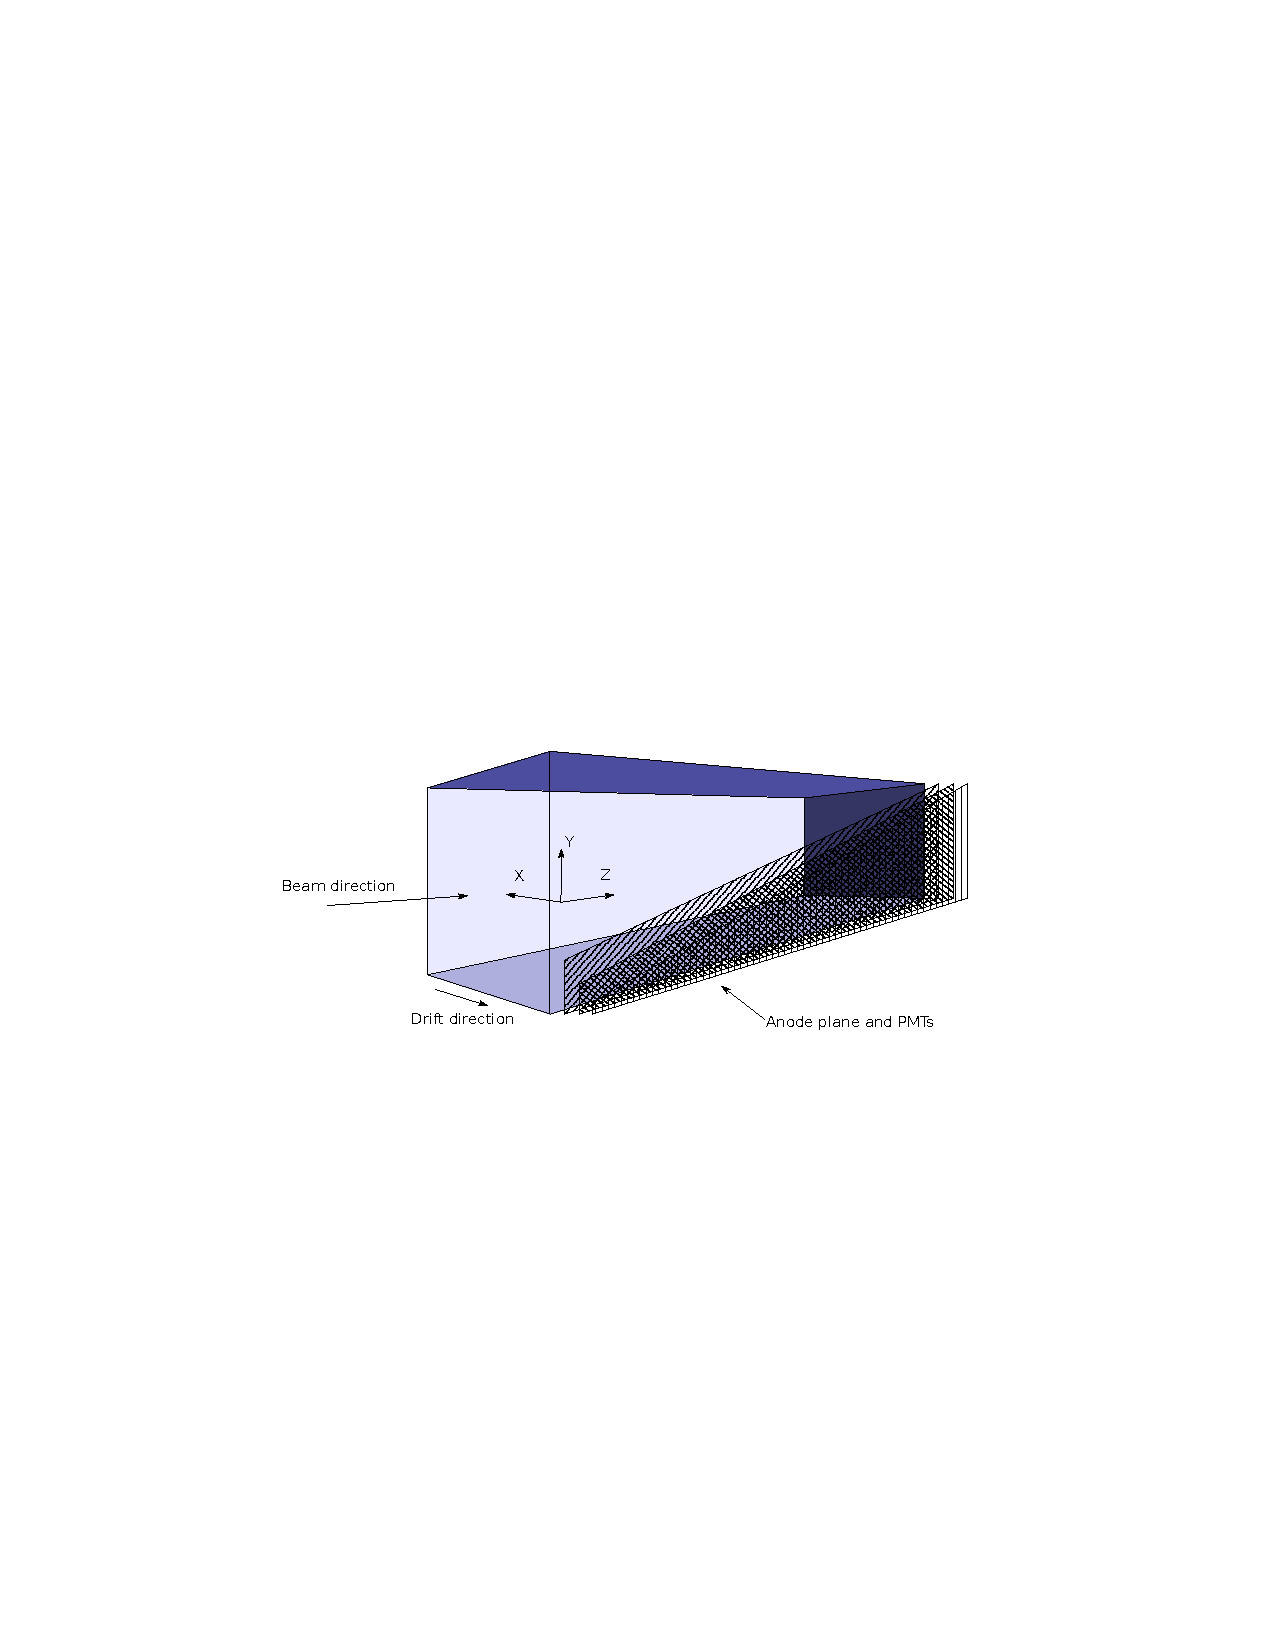
\includegraphics[width=0.8\linewidth]{figures/coord.pdf}

    \caption{The MicroBooNE coordinate system. The three wire planes are vertical (collection plane) and at  $\pm60^{\circ}$ to the vertical (induction planes). The dimensions of the TPC are 256.35 cm $\times$ 233 cm $\times$ 1036.8 cm (x $\times$ y $\times$ z). The fiducial volume of the detector is 236.35 cm $\times$ 203 cm $\times$ 1026.8 cm. The coordinate system is explained in detail in \cite{mcdata}.} \label{fig:coord}
  \end{center}
\end{figure}

A set of 32 photomultiplier tubes (PMTs) and three wire planes with 3 mm spacing at angles of 0,  $\pm 60^{\circ}$ with respect to the vertical are located in the TPC for event reconstruction and the cathode plane operating voltage is -70 kV. In a neutrino interaction, a neutrino from the beam interacts with an argon nucleus and the charged outgoing secondary particles traverse the medium, losing energy and leaving an ionization trail. The resulting ionization electrons drift to the anode side of the TPC, containing the wire planes. The passage of these electrons near the wire planes induces a signal in them. These signals are used to create three distinct two-dimensional views (in terms of wire and time) of the event. Combining these wire signals with timing information from the PMTs allows for full three-dimensional reconstruction of the event. %The fiducial volume used in this analysis is defined as the full TPC volume reduced by 20 cm from both the cathode plane and the anode wire planes, by 26.5 cm from both the top and bottom walls of the TPC, by 20 cm from the beam-upstream wall of the TPC, and by 36.8 cm from the beam-downstream wall of the TPC, which corresponds to a mass of 55 tons.

The Booster Neutrino Beam (BNB) is predominantly composed of muon neutrinos ($\nu_{\mu}$) with a peak neutrino energy of about 0.7 GeV, which can undergo charge-current ($\nu_{\mu}$CC) interactions in the TPC and produce muons. However, the abundant flux of cosmic muons, due to the shallow depth of the cryostat location (around 6 meters underground), can be a source of background to neutrino events and an optimal reconstruction of the cosmic rays in the TPC is of fundamental importance for the experiment. A Monte Carlo simulation of the the cosmic-ray flux hitting MicroBooNE gives a muon rate of 3.7 kHz, which corresponds to around 8 muons per DAQ time window.

This paper describes the work done to study the reconstruction efficiencies using a dataset of cosmic rays in the MicroBooNE TPC passing through the Muon Counter System (MuCS). The goal is to provide data and Monte Carlo reconstruction efficiencies that can be used to compare reconstruction performances and to show that an external cosmic-ray counter can be used to measure the data reconstruction efficiency in MicroBooNE.

We measured the data reconstruction efficiency comparing the number of events triggered by the MuCS and the number of events with a MuCS-compatible reconstructed track.
The Monte Carlo reconstruction efficiency, instead, was measured by comparing the number of generated cosmic rays with the number of reconstructed tracks, using simulated cosmic rays hitting the entire TPC.

The reconstruction efficiency is expressed as a function of the cosmic-ray starting angle (given by the spherical angles $\theta$ and $\phi$ relative to the orientation of the cosmic-ray trajectory) and of the expected length $L$ of its path in the TPC. More details on the Monte Carlo generation can be found in section \ref{sec:merging}.%, assuming it is a minimum-ionizing particle (MIP).

Using the \texttt{pan\-do\-ra\-Co\-smic} algorithm \cite{pandoracosmic} provided by the Pandora framework \cite{pandora}, the overall reconstruction efficiency is $96.1\pm0.1\thinspace(\mathrm{stat}) \pm 1.1\thinspace(\mathrm{sys})\thinspace\%$ for data and $96.3\pm0.1\thinspace\%$ for Monte Carlo.

In the future, the method described in this paper will be adapted to use the data coming form the Cosmic Ray Tagger \cite{crt}, which is able to tag around 80\% of the cosmic rays hitting MicroBooNE LArTPC. In this way, we will be able to cover the entire $(\theta,\phi,L)$ parameter space and measure efficiency-corrected quantities, such as the cosmic-ray flux in the LArTPC.


\section{The Muon Counter System}\label{sec:proc}
The MuCS, described in detail in \cite{mucs}, consists of two sets of planar modules made up of scintillator strips placed into two separate, light-tight panels, readout via wavelength shifting fibers connected to Multi-Anode PMTs and placed on the top of the TPC. The Multi-Anode PMTs are readout by a DAQ system, separated from the DAQ system that reads out the TPC and PMT systems of the main detector.

Each planar module is made up of two sets of 24 scintillator strips, 4 cm wide, arranged into bi-layers oriented perpendicular to each other. This configuration provides two coordinates ($z$ and $x$ in the MicroBooNE TPC coordinate system, shown in figure \ref{fig:coord}) of the crossing points of the cosmic rays. Combining these two coordinates with the height of the modules (corresponding to the $y$ coordinate in the MicroBooNE TPC coordinate system), it is possible to extrapolate the three-dimensional trajectory of the cosmic ray.

The starting angle of the cosmic ray, in spherical coordinates, will be given by:
\begin{align}
  \theta = \mathrm{acos}\left(\frac{z_{\mathrm{top}}-z_{\mathrm{bottom}}}{r}\right), \quad
  \phi = \mathrm{atan}\left(\frac{y_{\mathrm{top}}-y_{\mathrm{bottom}}}{x_{\mathrm{top}}-x_{\mathrm{bottom}}}\right),
\end{align}
where $r = \sqrt{(x_{\mathrm{top}}-x_{\mathrm{bottom}})^2+(y_{\mathrm{top}}-y_{\mathrm{bottom}})^2+(z_{\mathrm{top}}-z_{\mathrm{bottom}})^2}$ and the top (bottom) coordinates are given by the hits in the top (bottom) MuCS panel.


This analysis has been performed on three merged datasets, acquired with different geometrical configurations. For the three different configurations, the two panels have been placed at the upstream end, at the center and at the downstream end of MicroBooNE, respectively.
A three-dimensional schematic of the three MuCS setups is shown in figure \ref{fig:mucs}.

\begin{figure}[htbp]
  \begin{subfigure}{0.30\textwidth}
    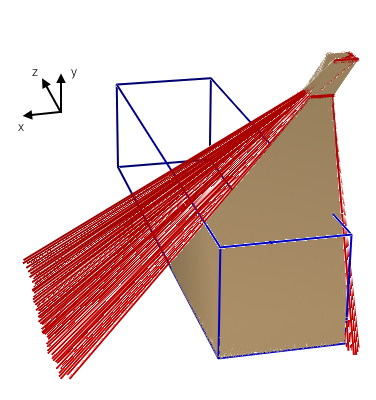
\includegraphics[width=\linewidth]{figures/upstream.png}
    \caption{Upstream} \label{fig:upstream}
  \end{subfigure}
  \begin{subfigure}{0.30\textwidth}
    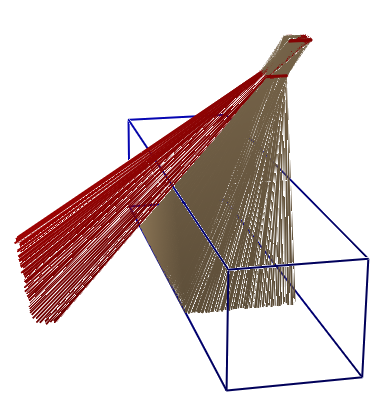
\includegraphics[width=\linewidth]{figures/center.png}
    \caption{Center} \label{fig:centre}
  \end{subfigure}
  \begin{subfigure}{0.30\textwidth}
    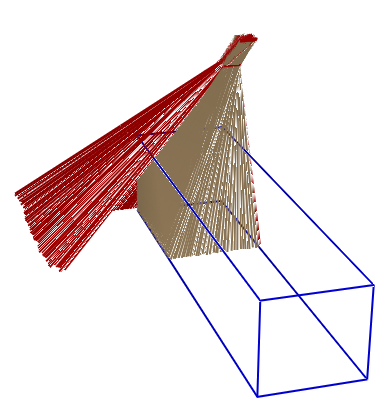
\includegraphics[width=\linewidth]{figures/downstream.png}
    \caption{Downstream} \label{fig:downstream}
  \end{subfigure}

  \caption{Monte Carlo simulation of the possible MuCS trajectories in the three different MuCS setups used in this analysis. Brown tracks correspond to cosmic rays hitting both MuCS panels and the TPC, while red tracks go through only the MuCS and miss the TPC.} \label{fig:mucs}
\end{figure}


\section{MuCS data and Monte Carlo processing}\label{sec:merging}
The MuCS is designed to provide a trigger on through-going muons that intersect two planes of scintillator strips. The trigger is propagated to the MicroBooNE trigger board to record a full TPC and PMT readout. With the MuCS trigger in place, the $t_0$ for a track associated with the MuCS is known and these tracks are useful for various detector physics and reconstruction studies.

The dataset used for this study has been collected with the DAQ configured in the trigger-readout mode: the MuCS trigger is sent to the TPC readout, while the MuCS DAQ saves the hit patterns seen in the scintillator strips.
The MuCS triggers at a rate of nearly 3 Hz.
Given a DAQ integration window of 100 ns, the accidental coincidental rate is negligible for our study. The probability that, during the same readout window (4.8 ms), another cosmic ray hits the MuCS is, given a trigger rate of 3 Hz, 0.01\% and it has also been considered negligible.

\subsection{Data sample generation}
The data then follows a processing path that merges the MuCS hit patterns and extrapolated trajectory information with the TPC and PMT data stream to form a MuCS-merged dataset. A flowchart of the procedure is shown in figure \ref{fig:scheme}.

\begin{figure}[htbp]
  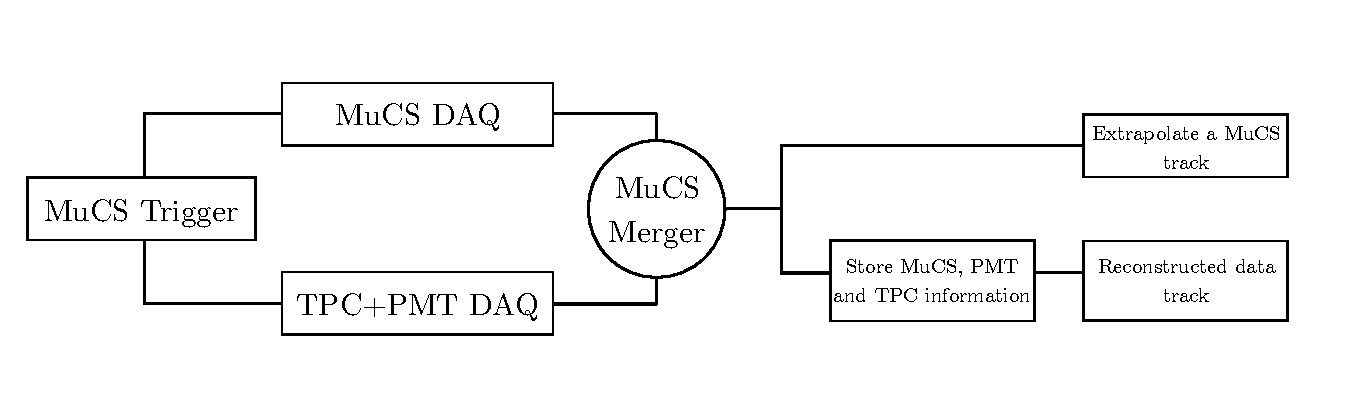
\includegraphics[width=\linewidth]{figures/scheme.pdf}
  \caption{Flowchart showing the procedure used to generate the dataset used in this analysis. We end up with two data products: one with extrapolated coordinates obtained using MuCS-only data and one with reconstructed TPC tracks and PMT flashes, if present.} \label{fig:scheme}
\end{figure}

The hits in the MuCS are used to obtain a point for each panel and extrapolate a track (MuCS-extrapolated track). The TPC hits, instead, are fed to the MicroBooNE reconstruction chain: the reconstructed track with the closest starting point to the intersection of the MuCS-extrapolated track with the TPC is stored in the dataset and it is defined as a MuCS-tagged track. The distance $d$ between these two points is defined as:
\begin{equation}\label{eq:d}
d = \sqrt{(x_{\mathrm{MuCS}}-x_{\mathrm{reco}})^2+(y_{\mathrm{MuCS}}-y_{\mathrm{reco}})^2+(z_{\mathrm{MuCS}}-z_{\mathrm{reco}})^2},
\end{equation}
where $(x_{\mathrm{MuCS}},y_{\mathrm{MuCS}},z_{\mathrm{MuCS}})$ and $(x_{\mathrm{reco}},y_{\mathrm{reco}},z_{\mathrm{reco}})$ are the coordinates of the intersection of the MuCS-extrapolated track with the TPC and of the start of the closest reconstructed track, respectively.
A PMT flash is associated with the MuCS signal if it falls between -1.0 and -0.8 \textmu s, where $t=0$ is given by the MuCS signal.
figure \ref{fig:evd} shows a diagram with the MuCS-tagged track, the MuCS-extrapolated track and the other reconstructed tracks in the same readout window.

\begin{figure}[htbp]
  \begin{center}
  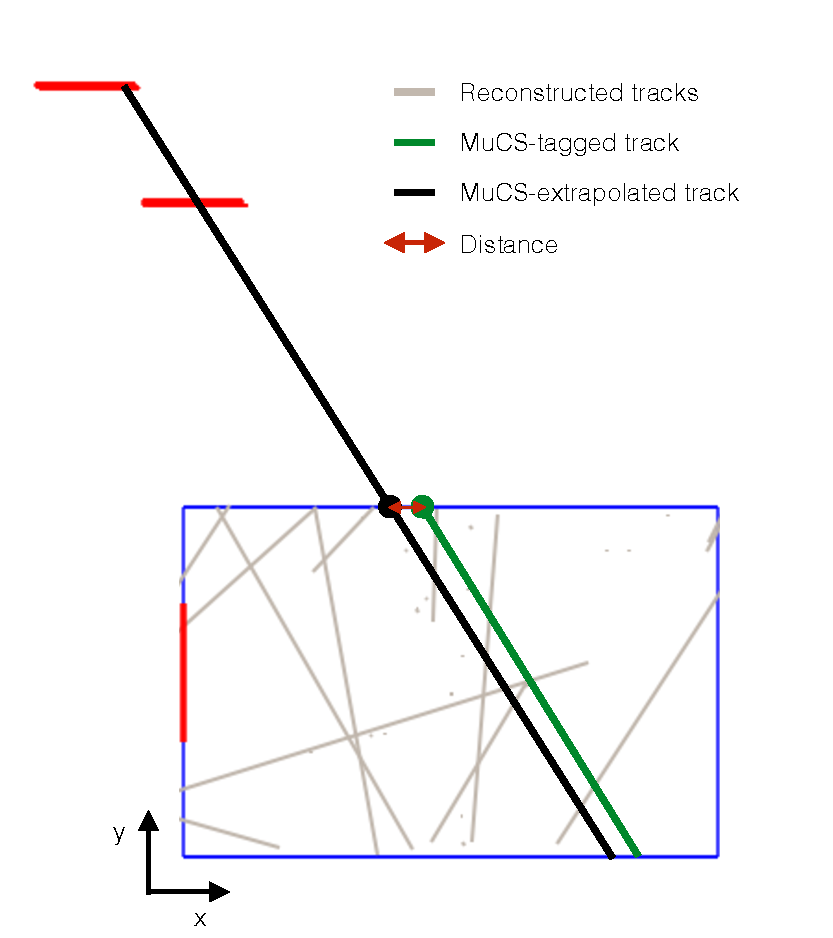
\includegraphics[width=0.50\linewidth]{figures/evd.pdf}  \vspace{1.8em}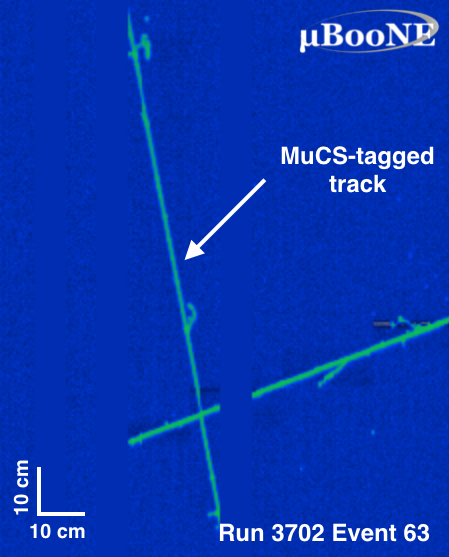
\includegraphics[width=0.40\linewidth]{figures/evd_display.png}

  \caption{Left: bi-dimensional view of a MuCS event. The black line shows the MuCS-extrapolated track, while the green line corresponds to the MuCS-tagged track. The black and green points correspond to the $(x_{\mathrm{MuCS}},y_{\mathrm{MuCS}},z_{\mathrm{MuCS}})$ and $(x_{\mathrm{reco}},y_{\mathrm{reco}},z_{\mathrm{reco}})$ coordinates, respectively. The red vertical line on the left border corresponds to the position of the PMT flash associated to the MuCS-tagged track. Right: corresponding portion of the event display for the collection plane, showing the MuCS-tagged track.} \label{fig:evd}
\end{center}
\end{figure}

Our dataset will then include two different sets of information, with a one-to-one correspondence:
\begin{itemize}
  \item MuCS-extrapolated information: using the two points given by the MuCS (one for each panel) we extrapolate a line crossing the entire TPC. In this way we obtain two extrapolated starting angles ($\theta$ and $\phi$), an extrapolated track length $L$ and extrapolated start/end points, using only MuCS information.
  \item Reconstructed TPC data information: for each event, we store the reconstructed spatial information of the MuCS-tagged track and of the in-time PMT flash, if present.
\end{itemize}

\subsection{Monte Carlo sample generation}

As Monte Carlo sample we used a complete cosmic-ray simulation, as described in \cite{cosmic}. The cosmic rays have been generated using CORSIKA \cite{corsika},  propagated with GEANT4 \cite{geant}, and then passed through the detector simulation stage. The detector simulation attempts to simulate the detector response as precisely as possible, meaning that the current state of the detector is reflected, including known unresponsive and noisy wires. Other known effects, such as the space charge effect \cite{sce}, are not currently modeled in the simulation.

The spherical angles $\theta$ and $\phi$ are measured using the starting point in the TPC and direction of the generated cosmic ray, while the expected track length $L$ is measured extrapolating a line through the TPC.
The distance $d$ is defined in this case as:
\begin{equation}\label{eq:d_mc}
d = \sqrt{(x_{\mathrm{sim}}-x_{\mathrm{reco}})^2+(y_{\mathrm{sim}}-y_{\mathrm{reco}})^2+(z_{\mathrm{sim}}-z_{\mathrm{reco}})^2},
\end{equation}
where $(x_{\mathrm{sim}},y_{\mathrm{sim}},z_{\mathrm{sim}})$ and $(x_{\mathrm{reco}},y_{\mathrm{reco}},z_{\mathrm{reco}})$ are the coordinates of the intersection of the simulated cosmic-ray trajectory with the TPC and of the closest reconstructed track, respectively.

From this complete Monte Carlo simulation, then, we selected only the cosmic rays with a starting angle $(\theta,\phi)$ within the geometrical acceptance of the MuCS.

Our aim is to show that the reconstruction efficiency of simulated cosmic rays, generated all over the TPC, can be successfully compared to the data reconstruction efficiency, obtained placing a small muon counter system in three different places.

\section{Reconstruction efficiencies}\label{sec:reco}

We define the MuCS reconstruction efficiency $\epsilon$ as the ratio between the number of events with a reconstructed MuCS cosmic ray and the number of MuCS-triggered events:
\begin{equation}\label{eq:eff}
  \epsilon = \frac{\mathrm{N.~of~reco.~MuCS~cosmic\myhyphen ray~events}}{\mathrm{N.~of~MuCS~triggered~events}}.
\end{equation}
In a data sample it is not possible to distinguish a MuCS cosmic ray from a normal cosmic ray and we define the MuCS-tagged track as the reconstructed track with the closest starting point $(x_{\mathrm{reco}},y_{\mathrm{reco}},z_{\mathrm{reco}})$ to the extrapolated MuCS starting point $(x_{\mathrm{MuCS}},y_{\mathrm{MuCS}},z_{\mathrm{MuCS}})$. However, events without a reconstructed MuCS cosmic ray will always have at least another reconstructed cosmic ray, so it is necessary to set a maximum distance $d_{\mathrm{max}}$ between the two points, $(x_{\mathrm{reco}},y_{\mathrm{reco}},z_{\mathrm{reco}})$ and $(x_{\mathrm{MuCS}},y_{\mathrm{MuCS}},z_{\mathrm{MuCS}})$. The number of our events with a MuCS-tagged track will then depend on $d_{\mathrm{max}}$. The efficiency $\epsilon_{\mathrm{tag}}$ of the cut on $d_{\mathrm{max}}$ is defined as:
\begin{equation}
  \epsilon_{\mathrm{tag}}=\frac{\mathrm{N.~of~reco.~events~within~}d_{\mathrm{max}}}{\mathrm{N.~of~MuCS~triggered~events}}
\end{equation}
and can be measured both for our data sample and for our general Monte Carlo simulation, replacing $(x_{\mathrm{MuCS}},y_{\mathrm{MuCS}},z_{\mathrm{MuCS}})$ with $(x_{\mathrm{sim}},y_{\mathrm{sim}},z_{\mathrm{sim}})$.

In a Monte Carlo simulation of a MuCS run, instead, the truth information allows us to verify if the MuCS-tagged cosmic ray is a real MuCS cosmic ray, or if it is another reconstructed cosmic ray, which happens to be mis-identified due to the extrapolated starting point distance being closer than $d_{\mathrm{max}}$.
The purity $P$ of our Monte Carlo MuCS sample will be defined as the ratio between the number of events with a reconstructed MuCS cosmic ray inside the $d_{\mathrm{max}}$ cut and the number of events with a reconstructed cosmic ray inside the $d_{\mathrm{max}}$ cut (MuCS-tagged cosmic rays):
\begin{equation}
  P=\frac{\mathrm{N.~of~reco.~MuCS~cosmic\myhyphen ray~events~within~}d_{\mathrm{max}}}{\mathrm{N.~of~reco.~events~within~}d_{\mathrm{max}}}.
\end{equation}
The acceptance $A$ of our cut on $d_{\mathrm{max}}$ will be defined as the ratio between the number of events with a reconstructed MuCS cosmic ray inside the $d_{\mathrm{max}}$ cut and the total number of events with a reconstructed MuCS cosmic ray:
\begin{equation}
  A=\frac{\mathrm{N.~of~reco.~MuCS~cosmic\myhyphen ray~events~within~}d_{\mathrm{max}}}{\mathrm{N.~of~reco.~MuCS~cosmic\myhyphen ray~events}}.
\end{equation}

figure \ref{fig:purity} shows the tagging efficiency $\epsilon_{\mathrm{tag}}$, the purity $P$ and the acceptance $A$ as a function of $d_{\mathrm{max}}$. The reconstruction efficiency $\epsilon$, which does not depend on $d_{\mathrm{max}}$, is also shown as a reference.

\begin{figure}[htbp]
  \begin{center}
    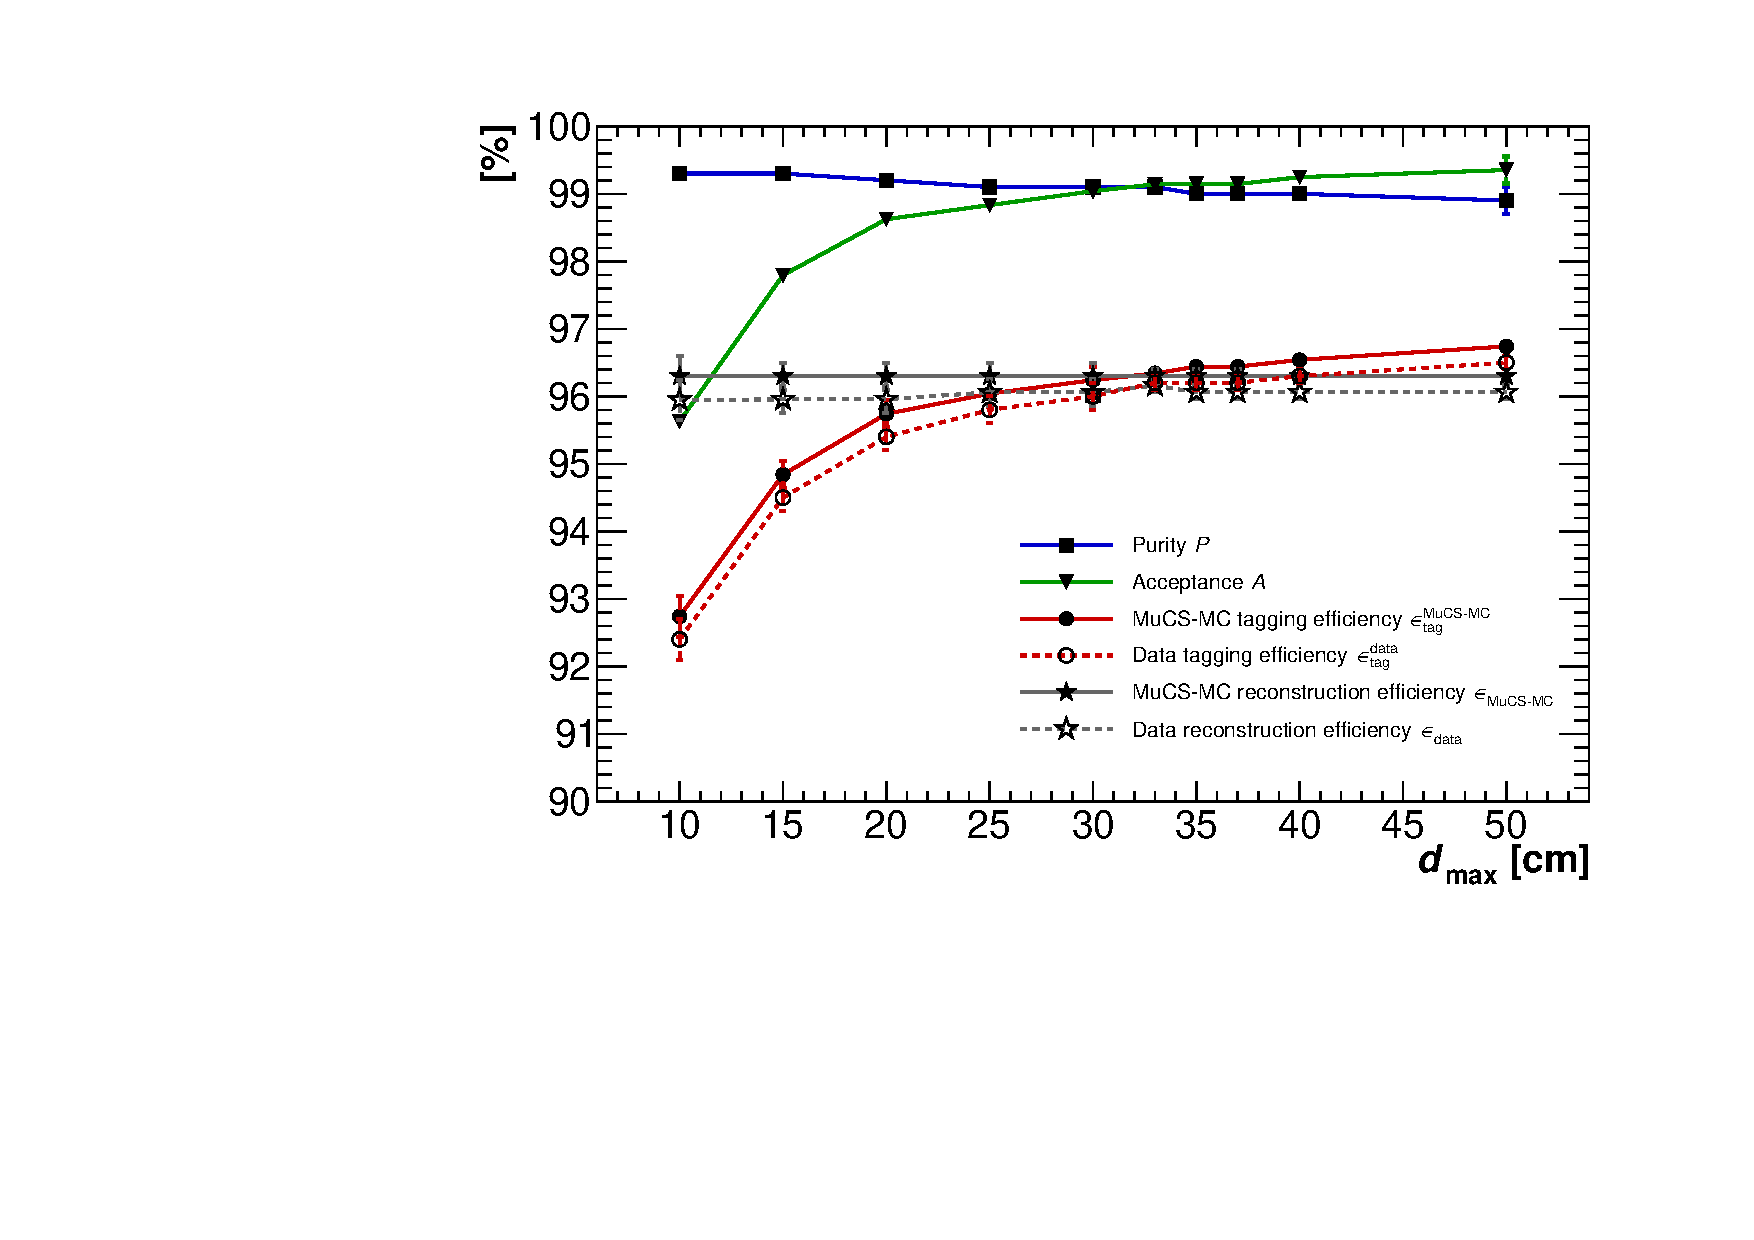
\includegraphics[width=0.7\linewidth]{figures/purity.pdf}
    \caption{Tagging efficiency $\epsilon_{\mathrm{tag}}$ (red), purity $P$ (blue) and acceptance $A$ (green) as a function of $d_{\mathrm{max}}$. The reconstruction efficiency $\epsilon$, which does not depend on $d_{\mathrm{max}}$, is also shown as a reference (dashed line).} \label{fig:purity}
  \end{center}
\end{figure}

The MuCS reconstruction efficiency, as defined in eq. \eqref{eq:eff}, can then be obtained by:
\begin{equation}
  \epsilon = \epsilon_{\mathrm{tag}} \times P / A,
\end{equation}
where the $P/A$ ratio will be taken from the MuCS Monte Carlo simulation, while $\epsilon_{\mathrm{tag}}$ can be measured with the data or with the general Monte Carlo simulation (described in section \ref{sec:merging}).
Using this formula, our data and Monte Carlo reconstruction efficiencies will not depend on the chosen value of $d_{\mathrm{max}}$. For convenience's sake, we chose a value of $d_{\mathrm{max}}$ that corresponds to $P/A = 1$, which in our case resulted to be $d_{\mathrm{max}}=32~\mathrm{cm}$.

It is now possible to measure the data and the Monte Carlo reconstruction efficiencies and express them as a function of the spherical starting angles $\theta$, $\phi$ and of the expected track length $L$ in the TPC. In an ideal TPC, in fact, the reconstruction efficiency for a cosmic ray depends only on the number of hit wires, which is given univocally by the direction and the length of the track in the TPC.

Our efficiency can then be plotted as a three-dimensional histogram: each bin will correspond to a particular combination of the $\theta$, $\phi$, $L$ variables. Bin width has been chosen large enough to have at least 15 MuCS triggered events in every ($\theta$, $\phi$, $L$) bin. The same $P/A$ correction factor has been applied to every bin. Figure \ref{fig:3d} shows both the data and the Monte Carlo reconstruction efficiency, generated as described in section \ref{sec:merging}.

\begin{figure}[htbp]
  \begin{subfigure}{0.52\textwidth}
    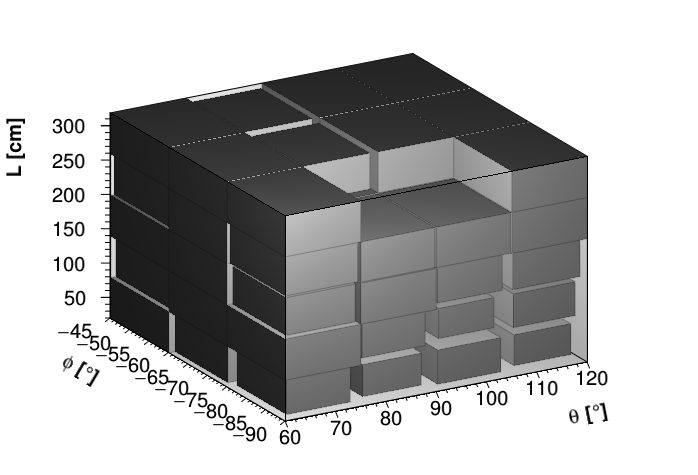
\includegraphics[width=\linewidth]{figures/3d_mc.png}
    \caption{Monte Carlo} \label{fig:3d_mc}
  \end{subfigure}
  \begin{subfigure}{0.52\textwidth}
    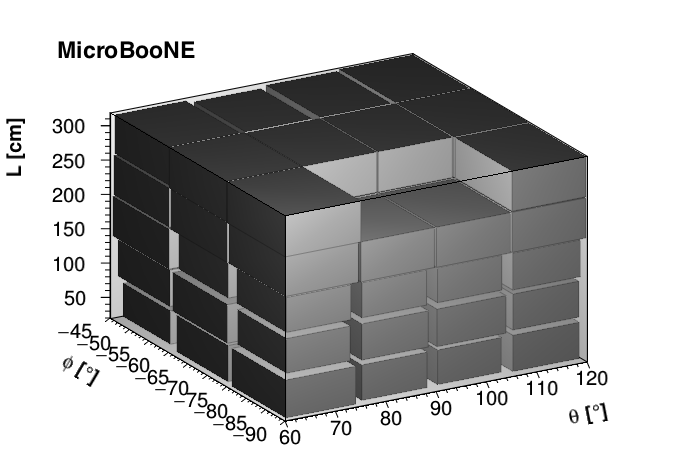
\includegraphics[width=\linewidth]{figures/3d_data.png}
    \caption{Data} \label{fig:3d_data}
  \end{subfigure}
  \caption{Monte Carlo and data three-dimensional reconstruction efficiency as a function of the starting angles $\theta$, $\phi$ and the extrapolated track length $L$. A larger box corresponds to a larger efficiency. The empty region in the upper part of the plot corresponds to a region of the parameter space not covered by our dataset.}\label{fig:3d}
\end{figure}

\subsection{Detector non-uniformities}\label{sec:wires}
The presence of detector non-uniformities can introduce a systematic error in the measurement of the reconstruction efficiency. In particular, the presence of noisy or unresponsive wires in specific regions of the detector can lower the reconstruction efficiency in some of our three dataset. However, the different configurations allow us to cover different regions of the TPC, providing information on potential non-uniformities.

To check if these non-uniformities introduce a systematic effect, we measured the significance $\sigma$ of the differences between the data reconstruction efficiencies measured in two different configurations with the following definition:
\begin{equation}
\sigma = \frac{\epsilon_a-\epsilon_b}{\sqrt{\Delta \epsilon_{a}^2 + \Delta \epsilon_b^2}},
\end{equation}
where $\epsilon_{a}$ ($\epsilon_{b}$) is the reconstruction efficiency in the $a$ ($b$) configuration and $\Delta \epsilon_{a}$ ($\Delta \epsilon_{b}$) is the corresponding statistical error. This significance has been measured for each $\theta,\phi,L$ bin and for each possible combination of central, downstream and upstream configuration (described in section \ref{sec:proc}). If there is a systematic effect, the standard deviation of the significances distribution should be larger than the unity. In our case, as shown in figure \ref{fig:significance}, the Gaussian fit of the distribution gives $\sigma = 1.54\pm0.12$, so larger than 1.

\begin{figure}[htbp]
  \begin{center}
    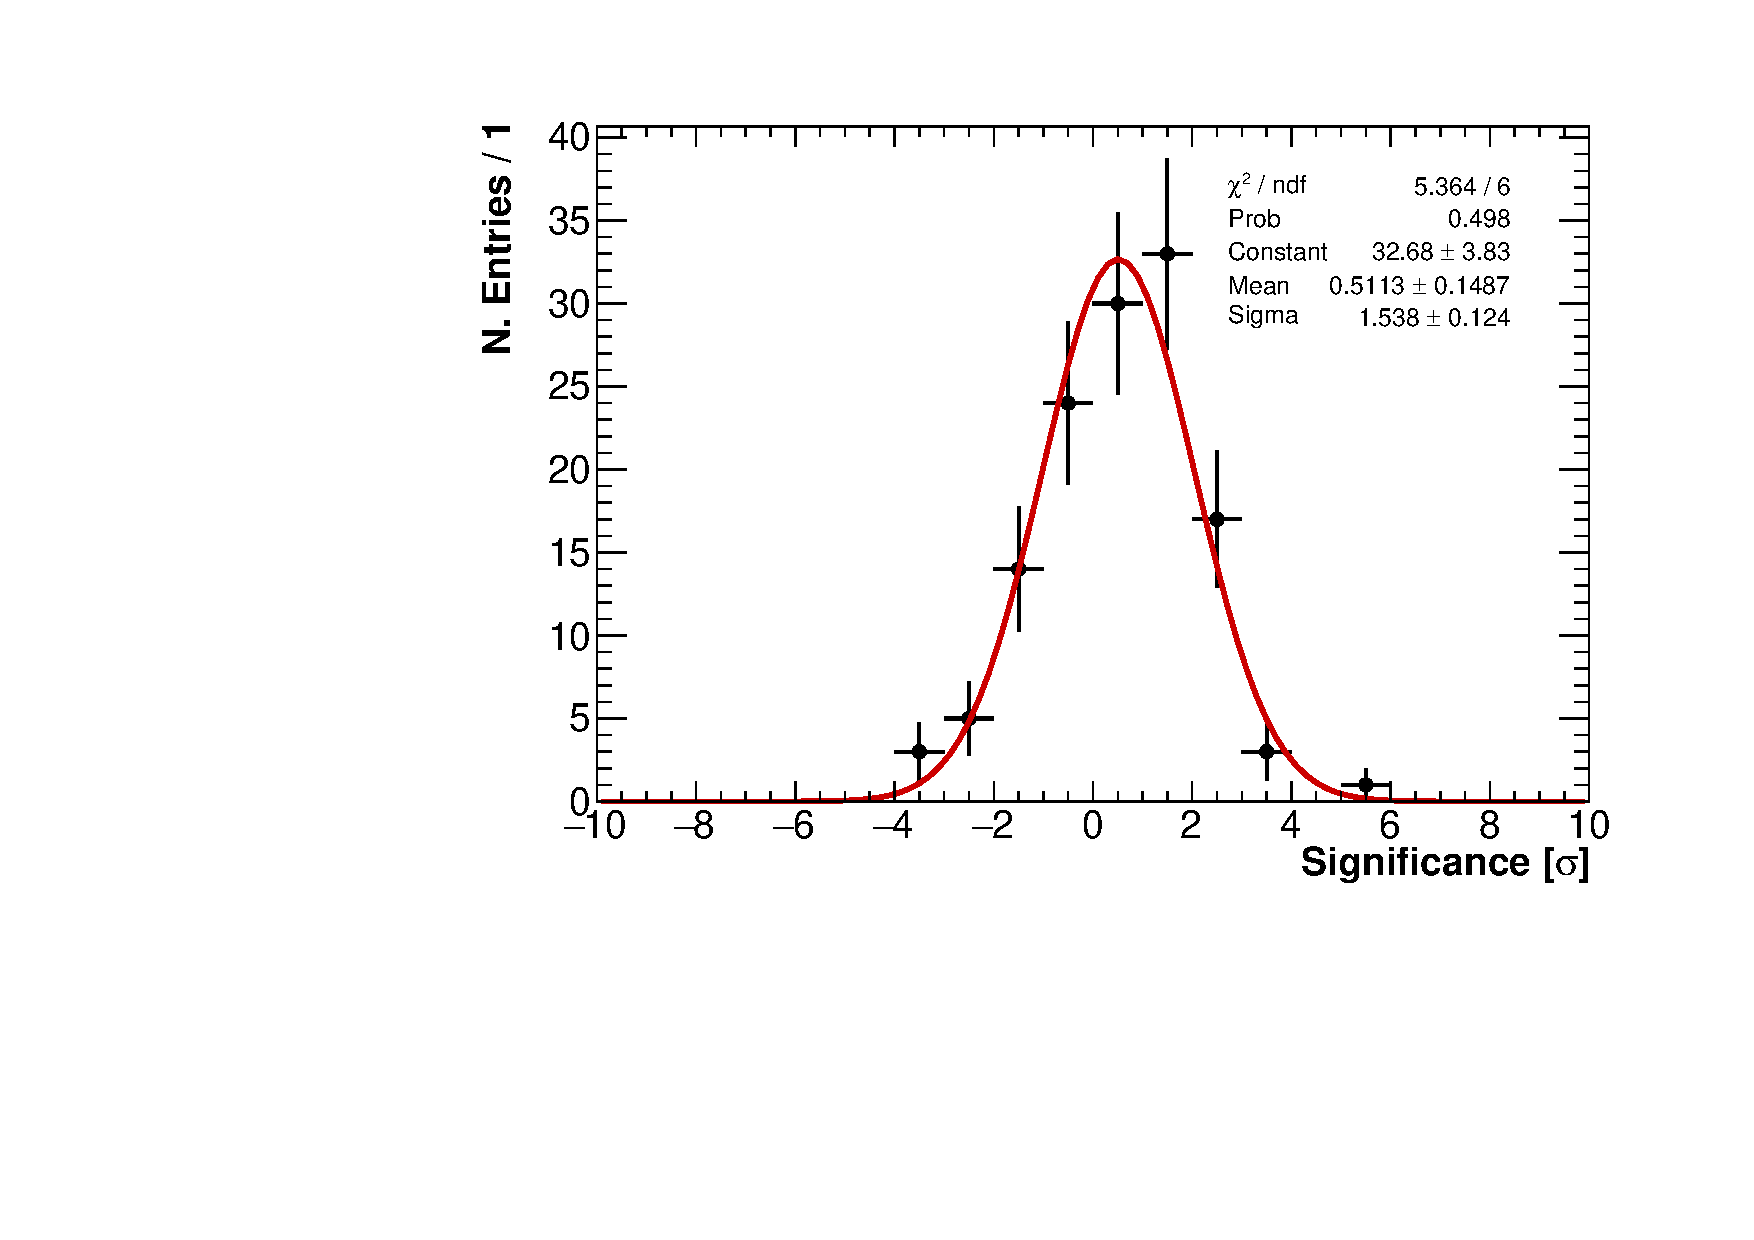
\includegraphics[width=0.7\linewidth]{figures/significance.pdf}
    \caption{Distribution of the significances of the reconstruction efficiency for each $\theta,\phi,L$ bin, measured for any combination of the three MuCS configuration.} \label{fig:significance}
  \end{center}
\end{figure}

In order to understand if these discrepancies are caused by noisy or unresponsive wires in specific parts of detector, the bins corresponding to significances larger than 3 have been reported in Tab. \ref{tab:significance}.

\begin{table}[htbp]
  \centering
  \begin{tabular}{cccccccccccc}
    \toprule
    $\theta\thinspace[^\circ]$ & $\phi\thinspace[^\circ]$ & $L\thinspace[\mathrm{cm}]$ & \phantom{a} & \multicolumn{2}{c}{Central} & \phantom{a} & \multicolumn{2}{c}{Upstream} & \phantom{a} & \multicolumn{2}{c}{Downstream}\\
     \cmidrule{5-6} \cmidrule{8-9} \cmidrule{11-12}
      &  &  & & avg. & err. & & avg. & err. & & avg. & err.   \\
    \midrule
    75 & -60 & 20 & & \textbf{0.85} & \textbf{0.04} & & \textbf{0.85} & \textbf{0.02} & & 0.95 & 0.02\\
    90 & -90 & 140 & & 0.97 & 0.03 & & \textbf{0.70} & \textbf{0.07} & & 0.93 & 0.04\\
    90 & -90 & 200 & & 0.99 & 0.01 & & \textbf{0.96} & \textbf{0.01} & & 0.99 & 0.01\\
    90 & -60 & 140 & & 0.98 & 0.01 & & \textbf{0.96} & \textbf{0.01} & & 0.99 & 0.01\\
    90 & -60 & 200 & & 0.99 & 0.01 & & \textbf{0.96} & \textbf{0.01} & & 0.89 & 0.01\\

    \bottomrule
  \end{tabular}
  \caption{Reconstruction efficiency for each geometrical configuration with a difference significance larger than 3. The lowest value is reported in bold.}\label{tab:significance}
\end{table}

As we can see, the configuration with the lowest reconstruction efficiency in this cases is always the upstream one. The drawing of the extrapolated tracks with those specific $\theta,\phi,L$ coordinates shows that, for the upstream configuration, the corresponding cosmic rays go through regions with noisy or unresponsive wires in one of the induction planes (figure \ref{fig:wires}).

\begin{figure}[htbp]
  \begin{center}
    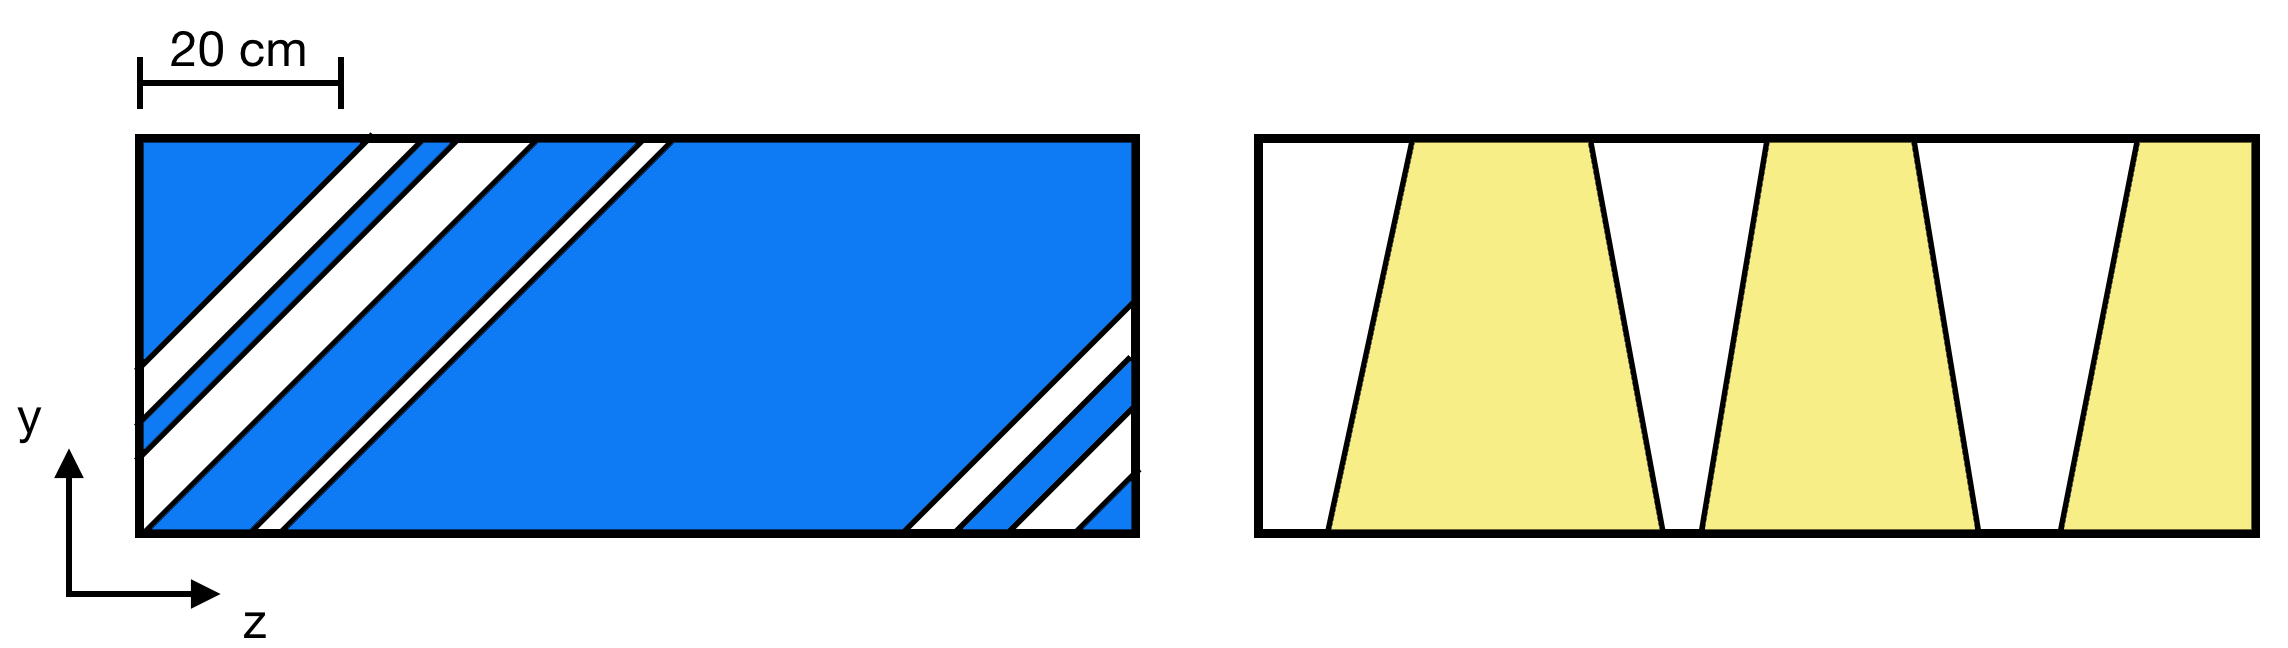
\includegraphics[width=1\linewidth]{figures/wire_tracks.png}
    \caption{Bi-dimensional plot of the average $dE/dx$, showing the regions with missing wires on one of the induction planes (left) and extrapolated tracks corresponding to the coordinates in Tab. \ref{tab:significance} (right). As we can see, the tracks in the upstream part of the detector (low $z$) go through a region with several missing wires.} \label{fig:wires}
  \end{center}
\end{figure}


Moreover, since their $\theta$ angle is close to $90^\circ$, they are also aligned with the wires of the collection plane. Thus, these cosmic rays have few hits in two of the three planes and the algorithm is not efficient to reconstruct a track. Figure \ref{fig:example} shows a non-reconstructed MuCS cosmic ray going through the region with missing wires and parallel to the collection plane wires.

\begin{figure}[htbp]
  \begin{center}
    \begin{subfigure}{0.3\textwidth}
      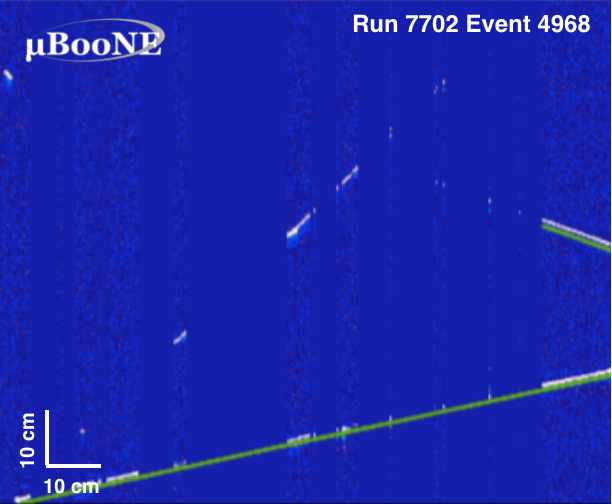
\includegraphics[width=\linewidth]{figures/u.png}
      \caption{Induction (U) plane} \label{fig:u}
    \end{subfigure}
    \begin{subfigure}{0.3\textwidth}
      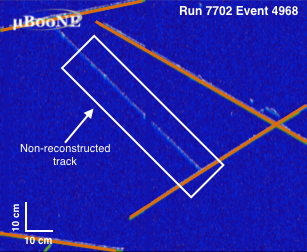
\includegraphics[width=\linewidth]{figures/v.png}
      \caption{Induction (V) plane} \label{fig:v}
    \end{subfigure}
    \begin{subfigure}{0.3\textwidth}
      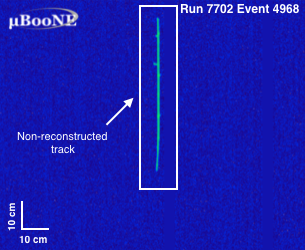
\includegraphics[width=\linewidth]{figures/y.png}
      \caption{Collection (Y) plane} \label{fig:y}
    \end{subfigure}    \caption{Event display of a non-reconstructed MuCS cosmic-ray track in the U, V and Y planes. Green lines correspond to the reconstructed tracks.} \label{fig:example}
  \end{center}
\end{figure}



We quote the systematic error related to the detector non-uniformities for each $\theta,\phi,L$ bin as the difference between the best reconstructing efficiency of the three configurations and the overall reconstruction efficiency (obtained merging the three dataset), a method described in \cite{besiii}.

%\subsection{Energy sampling}
%The multiple Coulomb scattering depends on the energy of the cosmic ray. The angular dispersion $\theta_{0}$ of a cosmic muon can be, in fact, calculated by the relation, expressed in \cite{pdg}:
%\begin{equation}
%\theta_{0} = \frac{13.6~\mathrm{MeV}}{\beta c p}\sqrt{x/X_{0}}\left[1+0.038\thinspace\mathrm{ln}(x/X_0)\right],
%\end{equation}
%where $p$ and $\beta c$ are the momentum and velocity of the incident particle, and $x/X_0$ is the thickness of the scattering medium in radiation lengths.

%\begin{figure}[htbp]
%  \begin{center}
%    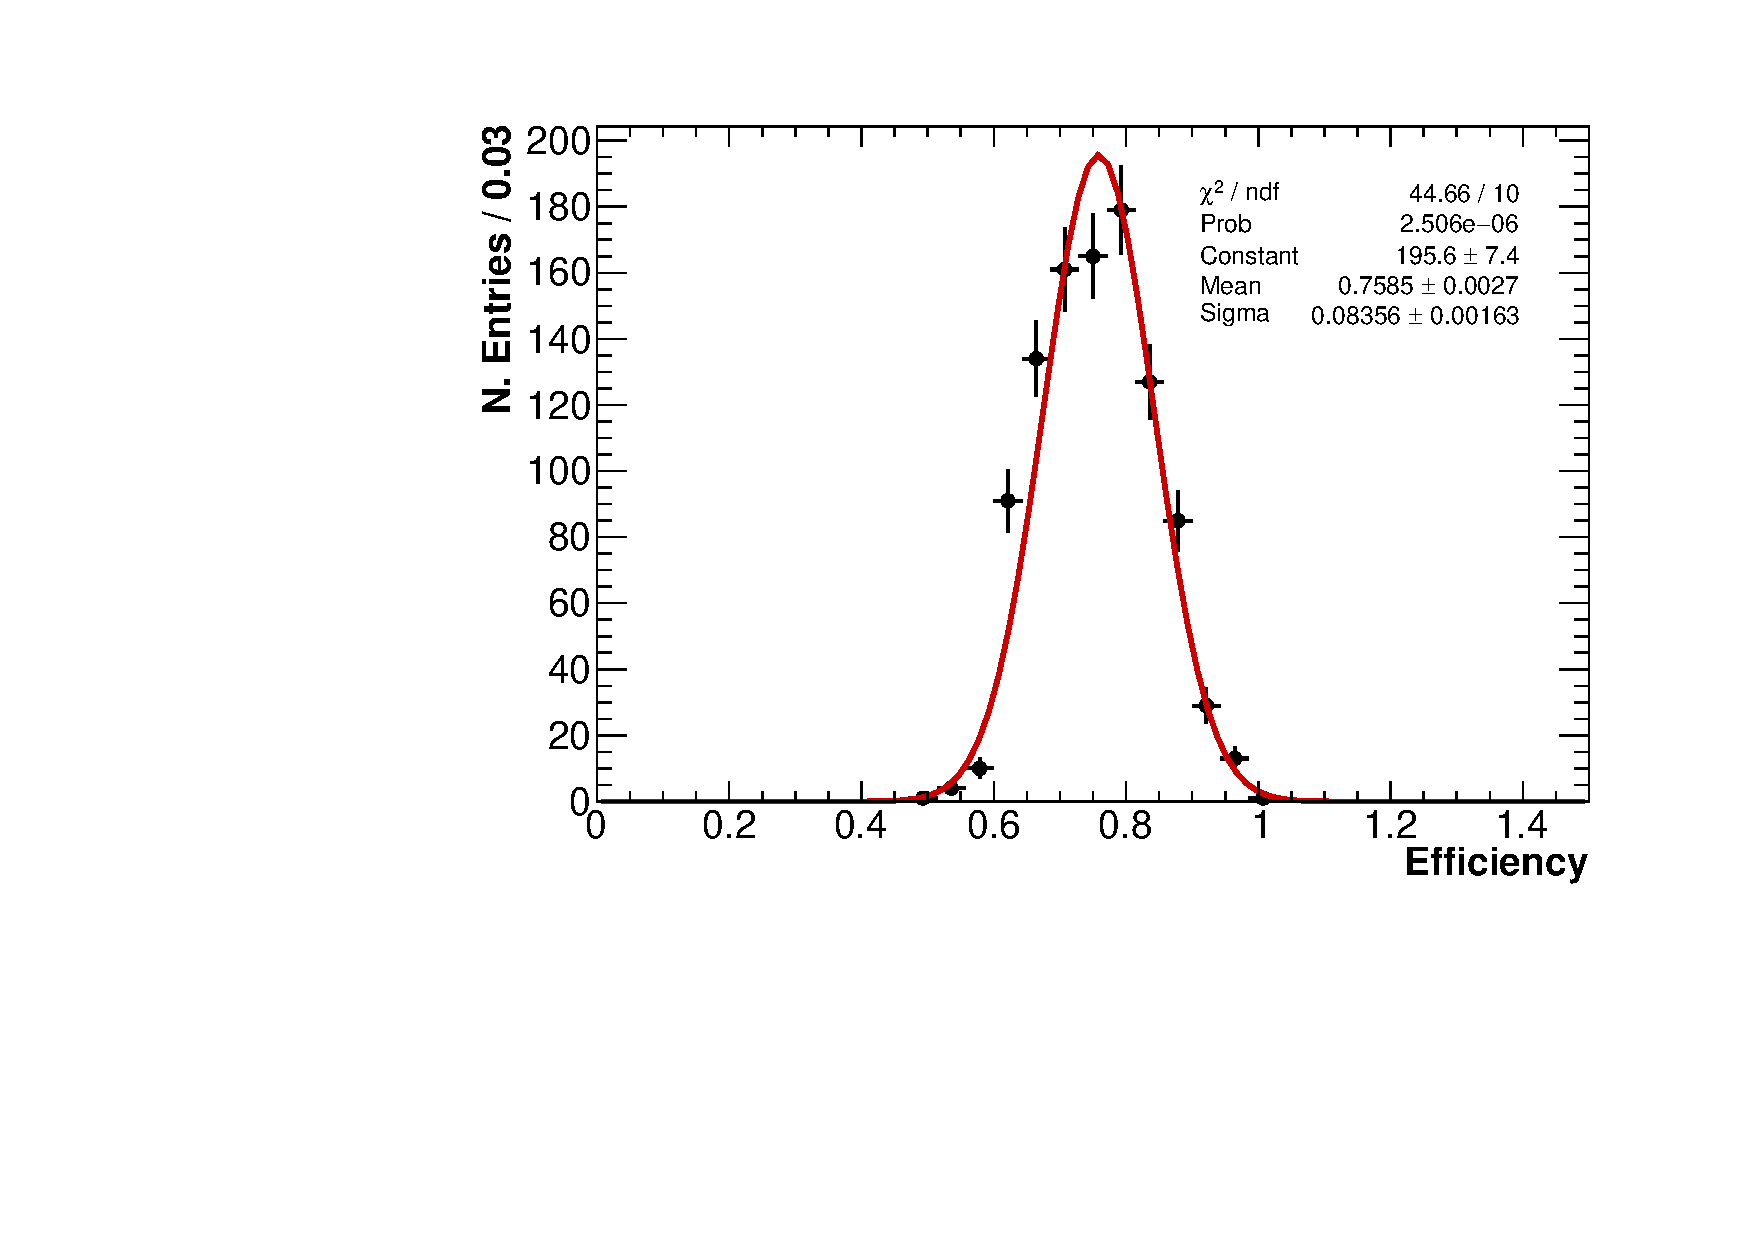
\includegraphics[width=0.7\linewidth]{figures/sampling.pdf}
%    \caption{Distribution of the reconstruction efficiency obtained generating 1000 thousand pseudo-experiments with 19 MuCS-triggered events each.} \label{fig:sampling}
%  \end{center}
%\end{figure}

%Thus, low-energy cosmic rays scatter more than high-energy ones and they have an higher probability to be further than $d_{\mathrm{max}}$ from the extrapolated starting point of the MuCS cosmic ray. In the bins where the data reconstruction efficiency has been measured with low statistics, then, it can happen to have MuCS cosmic rays distributed in a small region of the energy spectrum, biasing the measurement of the reconstruction efficiency.

%In order to verify if this sampling introduces a systematic effect, we choose the bin with the lowest number of MuCS events, which is 19. We then performed a Monte Carlo simulation, generating one thousand pseudo-experiments with 19 MuCS events sampled from the CORSIKA cosmic-ray energy spectrum with the same starting angles and length of our chosen bin. We filled an histogram with the value of the reconstruction efficiency for each pseudo-experiment and fitted the distribution with a Gaussian (figure \ref{fig:sampling}). The $\sigma$ of the fit is $0.084$, compatible with the statistical error of the same bin which is $0.083$. Thus, we conclude that the energy sampling of the cosmic rays does not introduce a systematic effect.

\subsection{Data/Monte Carlo comparison}
It is now possible to compare the data and Monte Carlo reconstruction efficiencies. The three-dimensional efficiency plots shown in figure \ref{fig:3d} can be projected on the bi-dimensional planes ($\theta,\phi$), ($\theta,L$), ($\phi,L$), shown in figure \ref{fig:2d} and on the single axis $\theta$, $\phi$, $L$, shown in figure \ref{fig:1d}.

\begin{figure}[htbp]
  \begin{center}
    \begin{subfigure}{0.6\textwidth}
      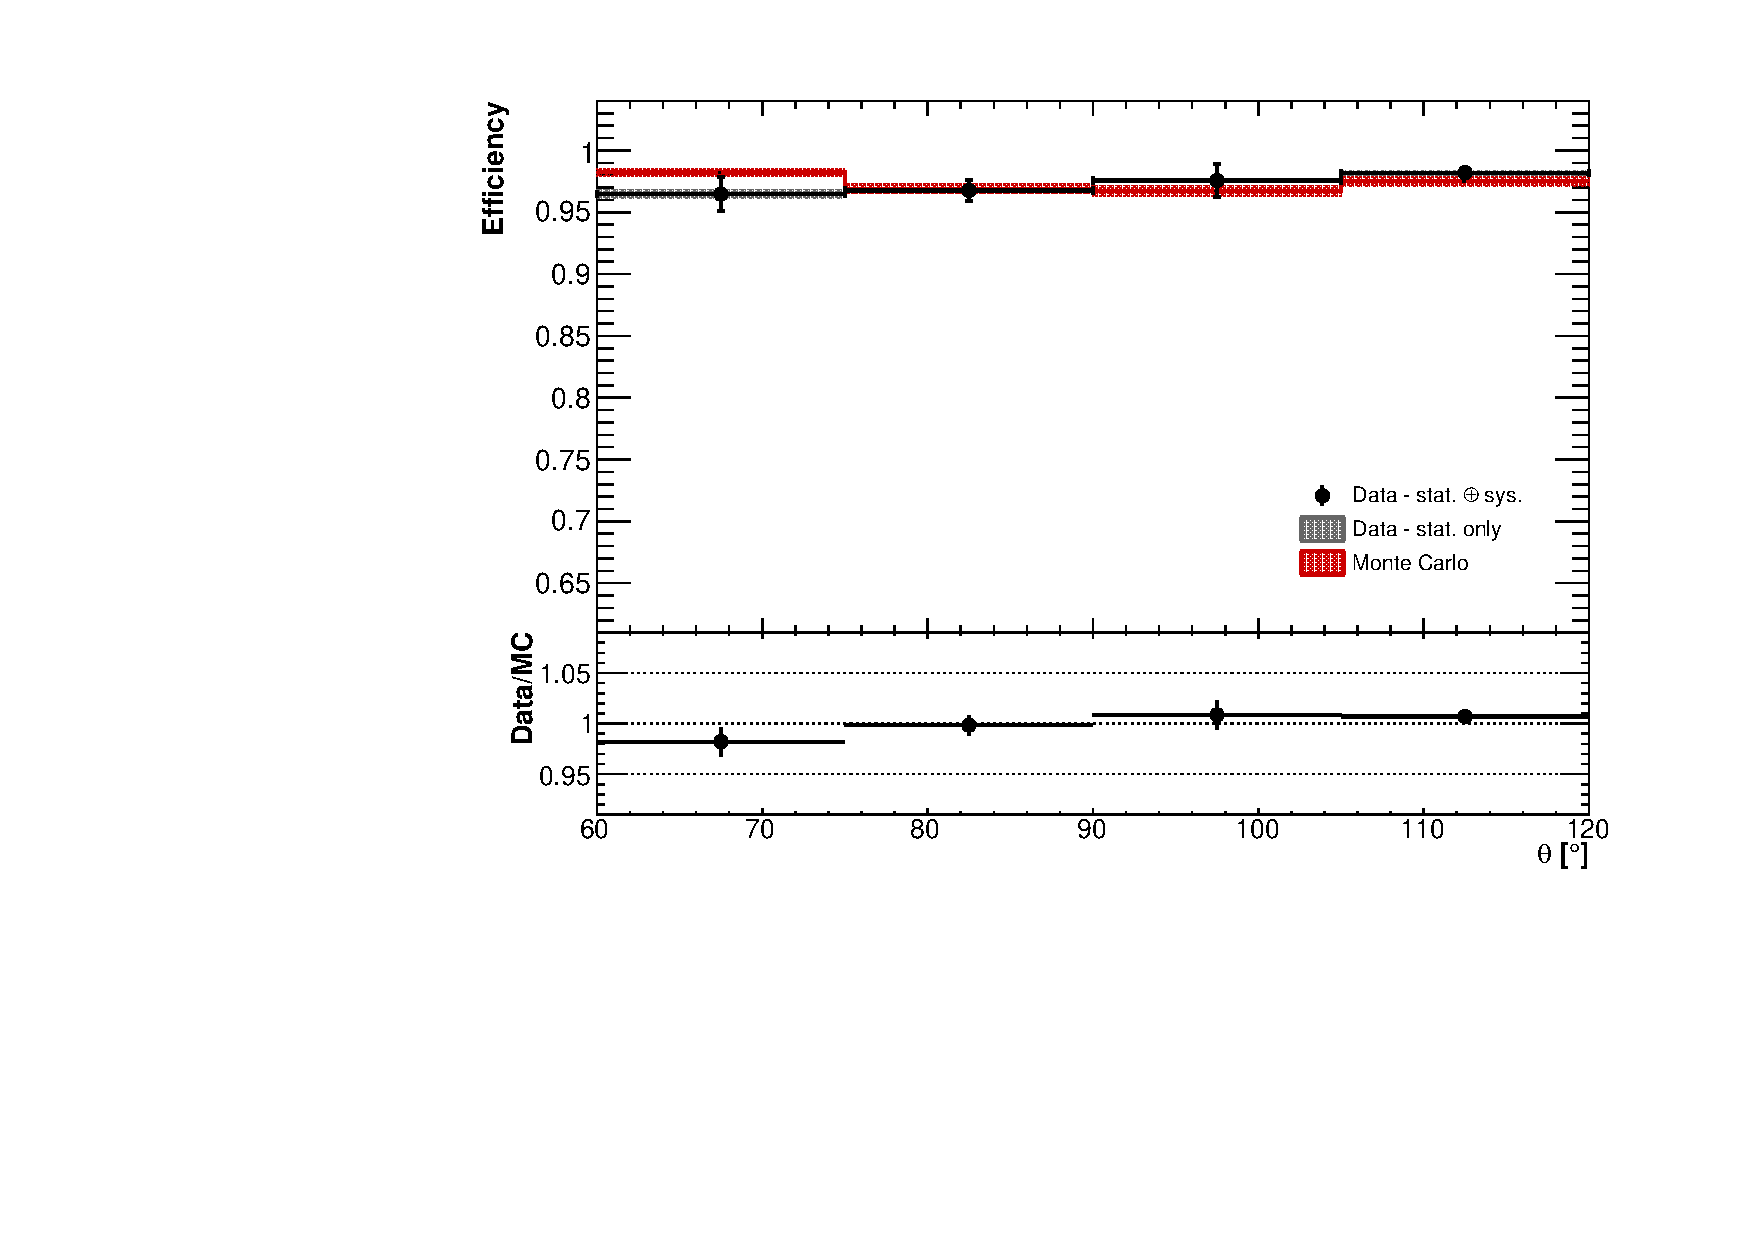
\includegraphics[width=\linewidth]{figures/theta.pdf}
      \caption{$\theta$} \label{fig:theta}
    \end{subfigure}
    \begin{subfigure}{0.6\textwidth}
      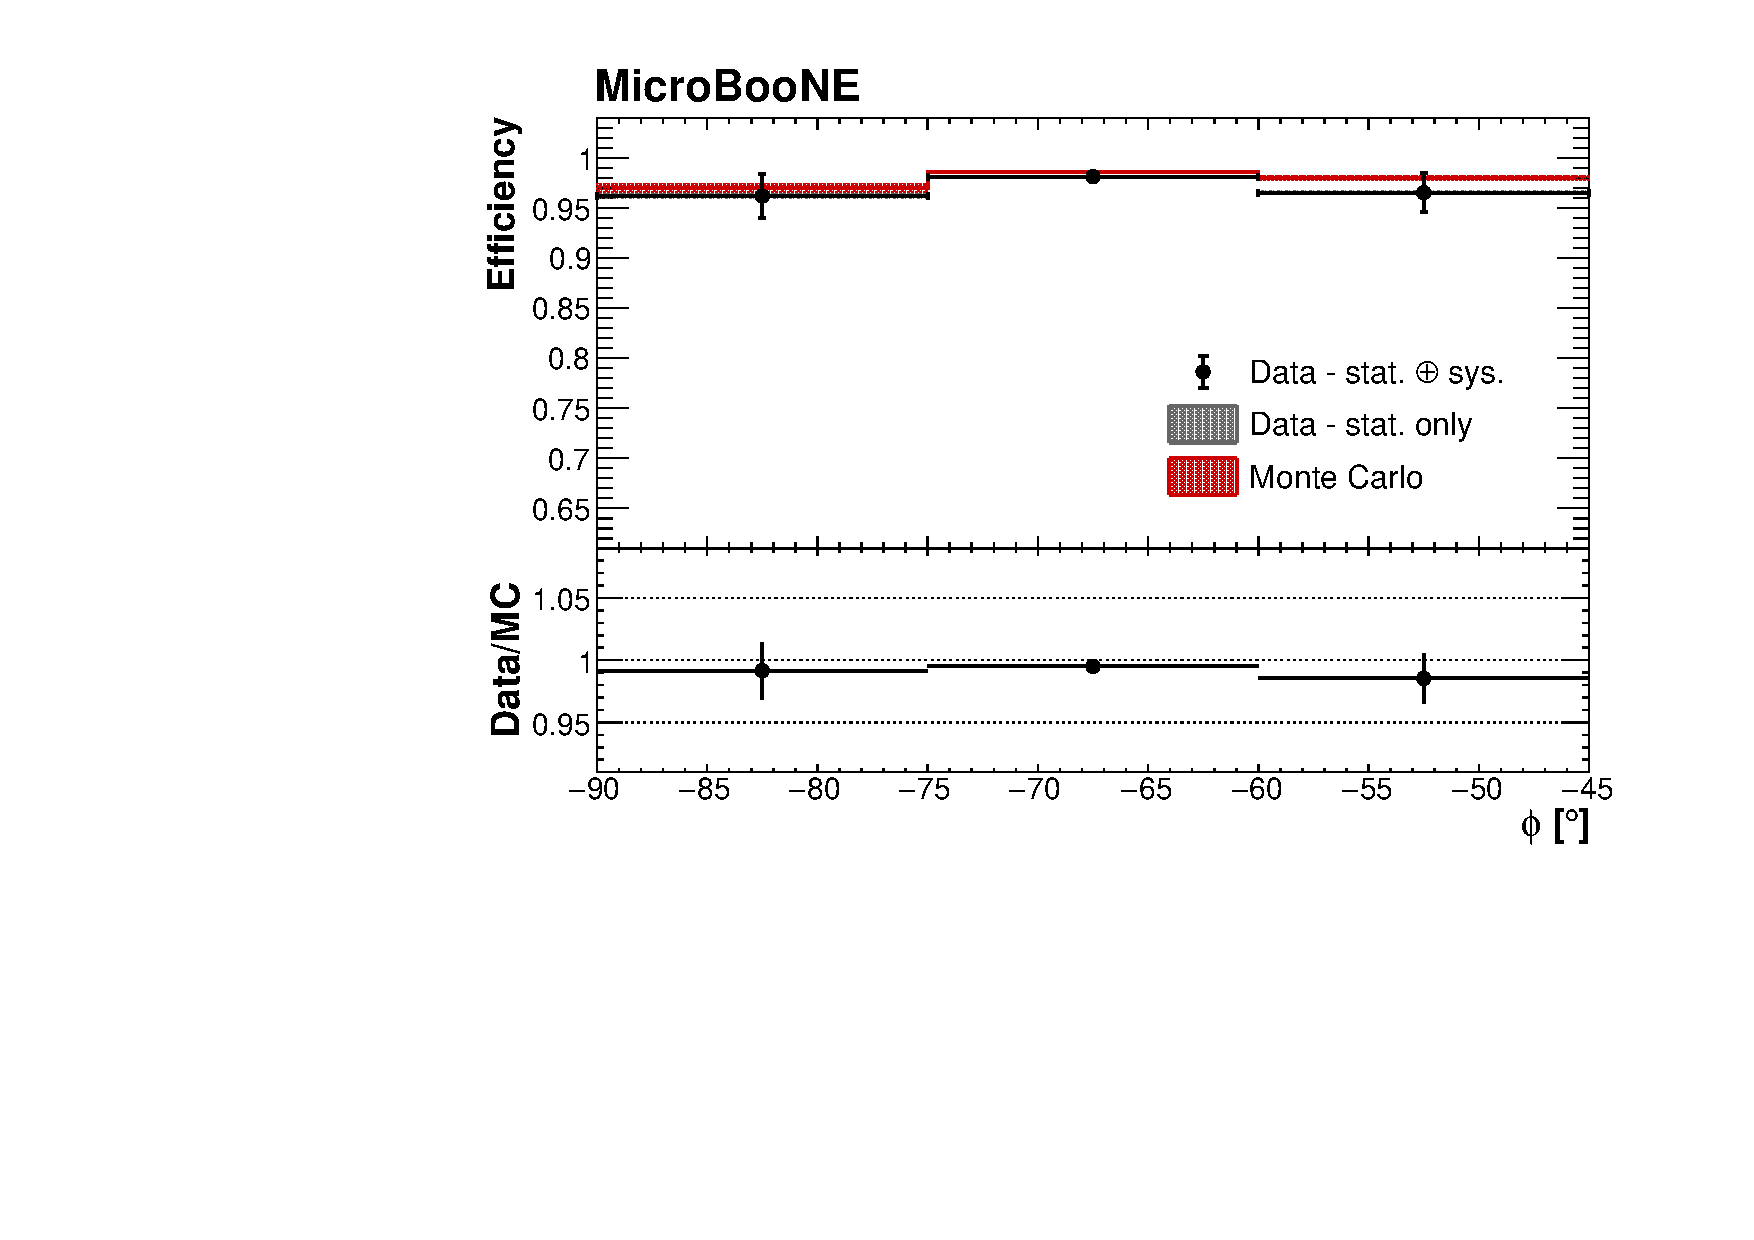
\includegraphics[width=\linewidth]{figures/phi.pdf}
      \caption{$\phi$} \label{fig:phi}
    \end{subfigure}
    \begin{subfigure}{0.6\textwidth}
      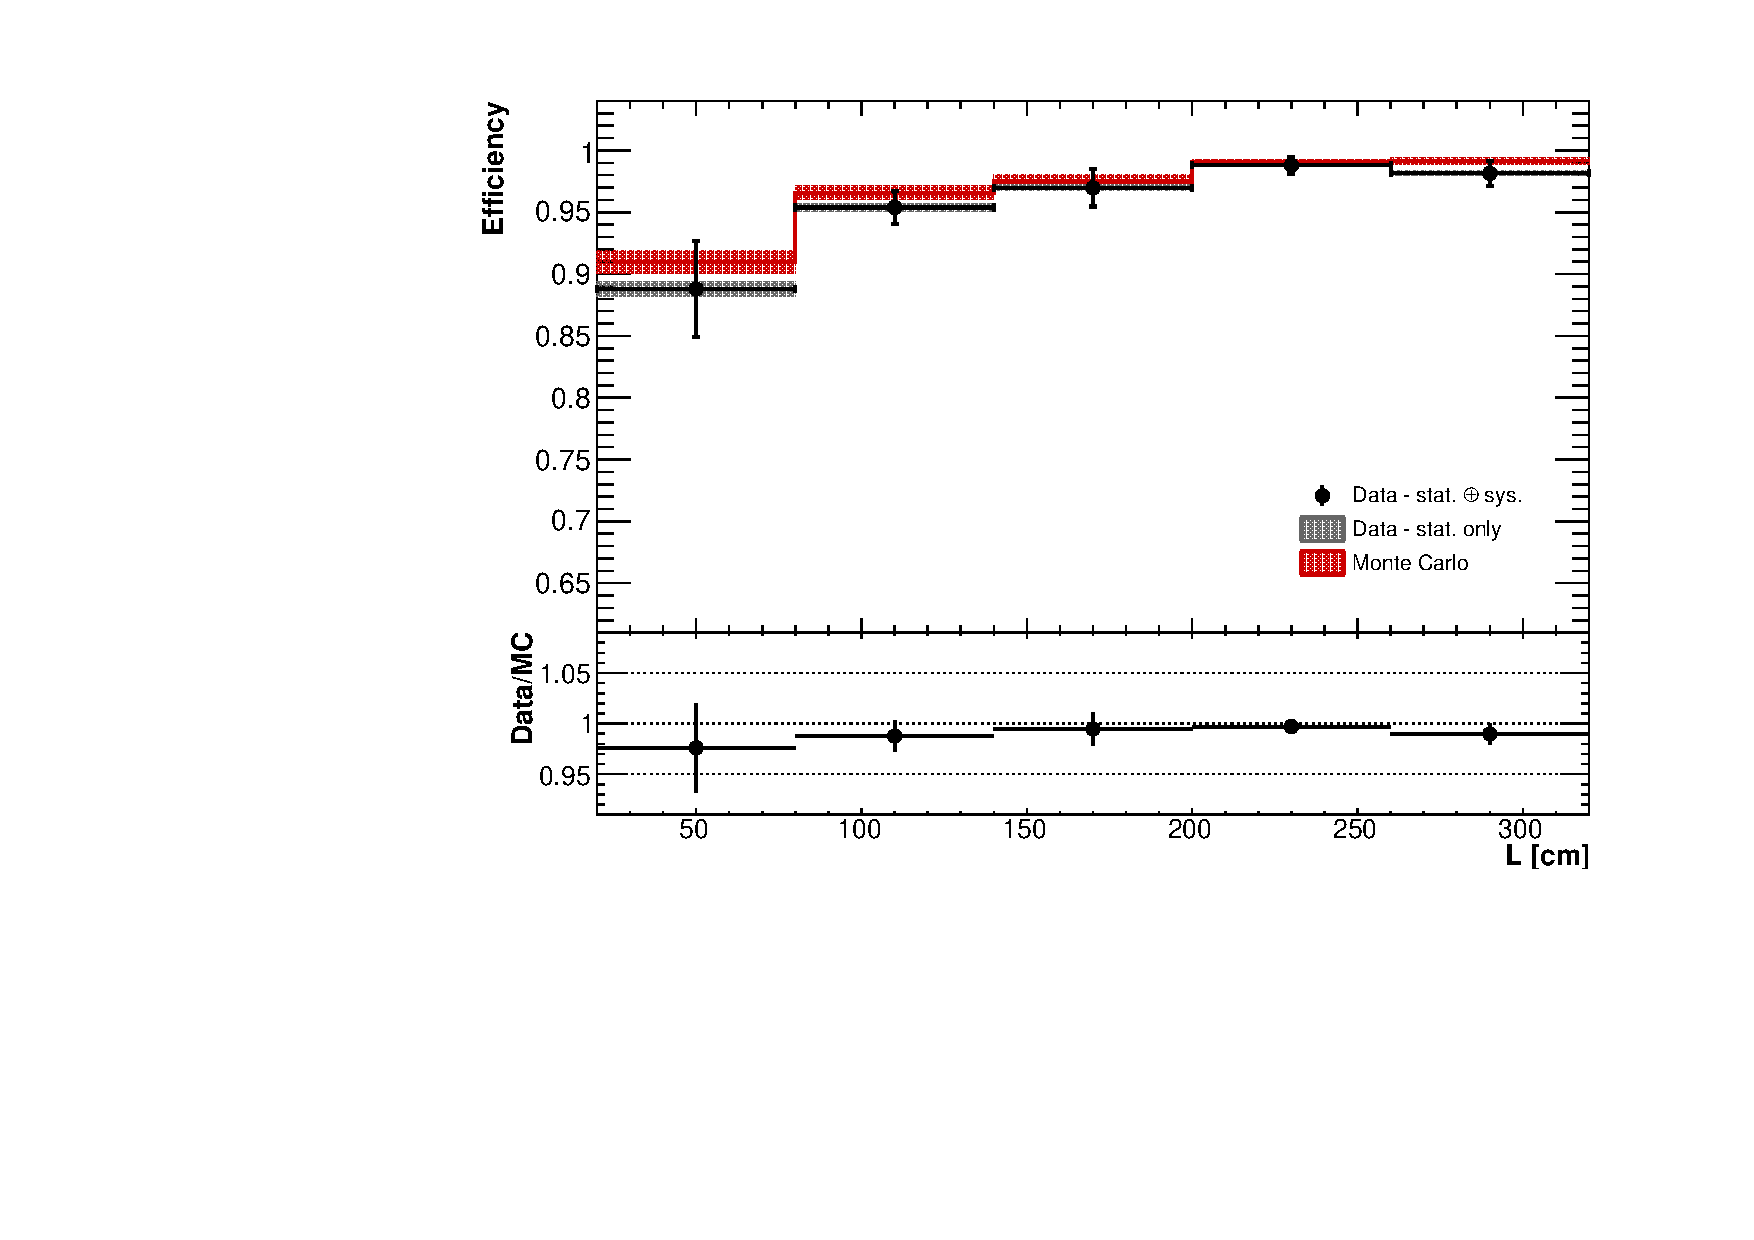
\includegraphics[width=\linewidth]{figures/l.pdf}
      \caption{$L$} \label{fig:l}
    \end{subfigure}
    \caption{Monte Carlo (red line) and data (black points) reconstruction efficiency as a function of the starting angles $\theta$, $\phi$ and the extrapolated track length $L$.}\label{fig:1d}
  \end{center}
\end{figure}

Taking into account the systematic error given by the detector non-uniformities, as described in section \ref{sec:wires}, the obtained data/Monte Carlo agreement is satisfactory, with almost every bin with a data/Monte Carlo ratio within 2$\sigma$ of unity. As expected, the reconstruction efficiency is proportional to the expected track length $L$ in the TPC, since longer tracks correspond, in general, to a larger number of hit wires and they are then easier to reconstruct.

The overall reconstruction efficiency, obtained integrating the three-dimensional plot, is:
\begin{align*}
\epsilon_{\mathrm{data}} &= 96.1 \pm 0.1~\mathrm{(stat)} \pm 1.1~\mathrm{(sys)}~\%\\
\epsilon_{\mathrm{MC}} &= 96.3 \pm 0.1~\%
\end{align*} for data and Monte Carlo, respectively. The agreement between the two values is within the error.



\begin{figure}[htbp]
  \begin{subfigure}{0.33\textwidth}
    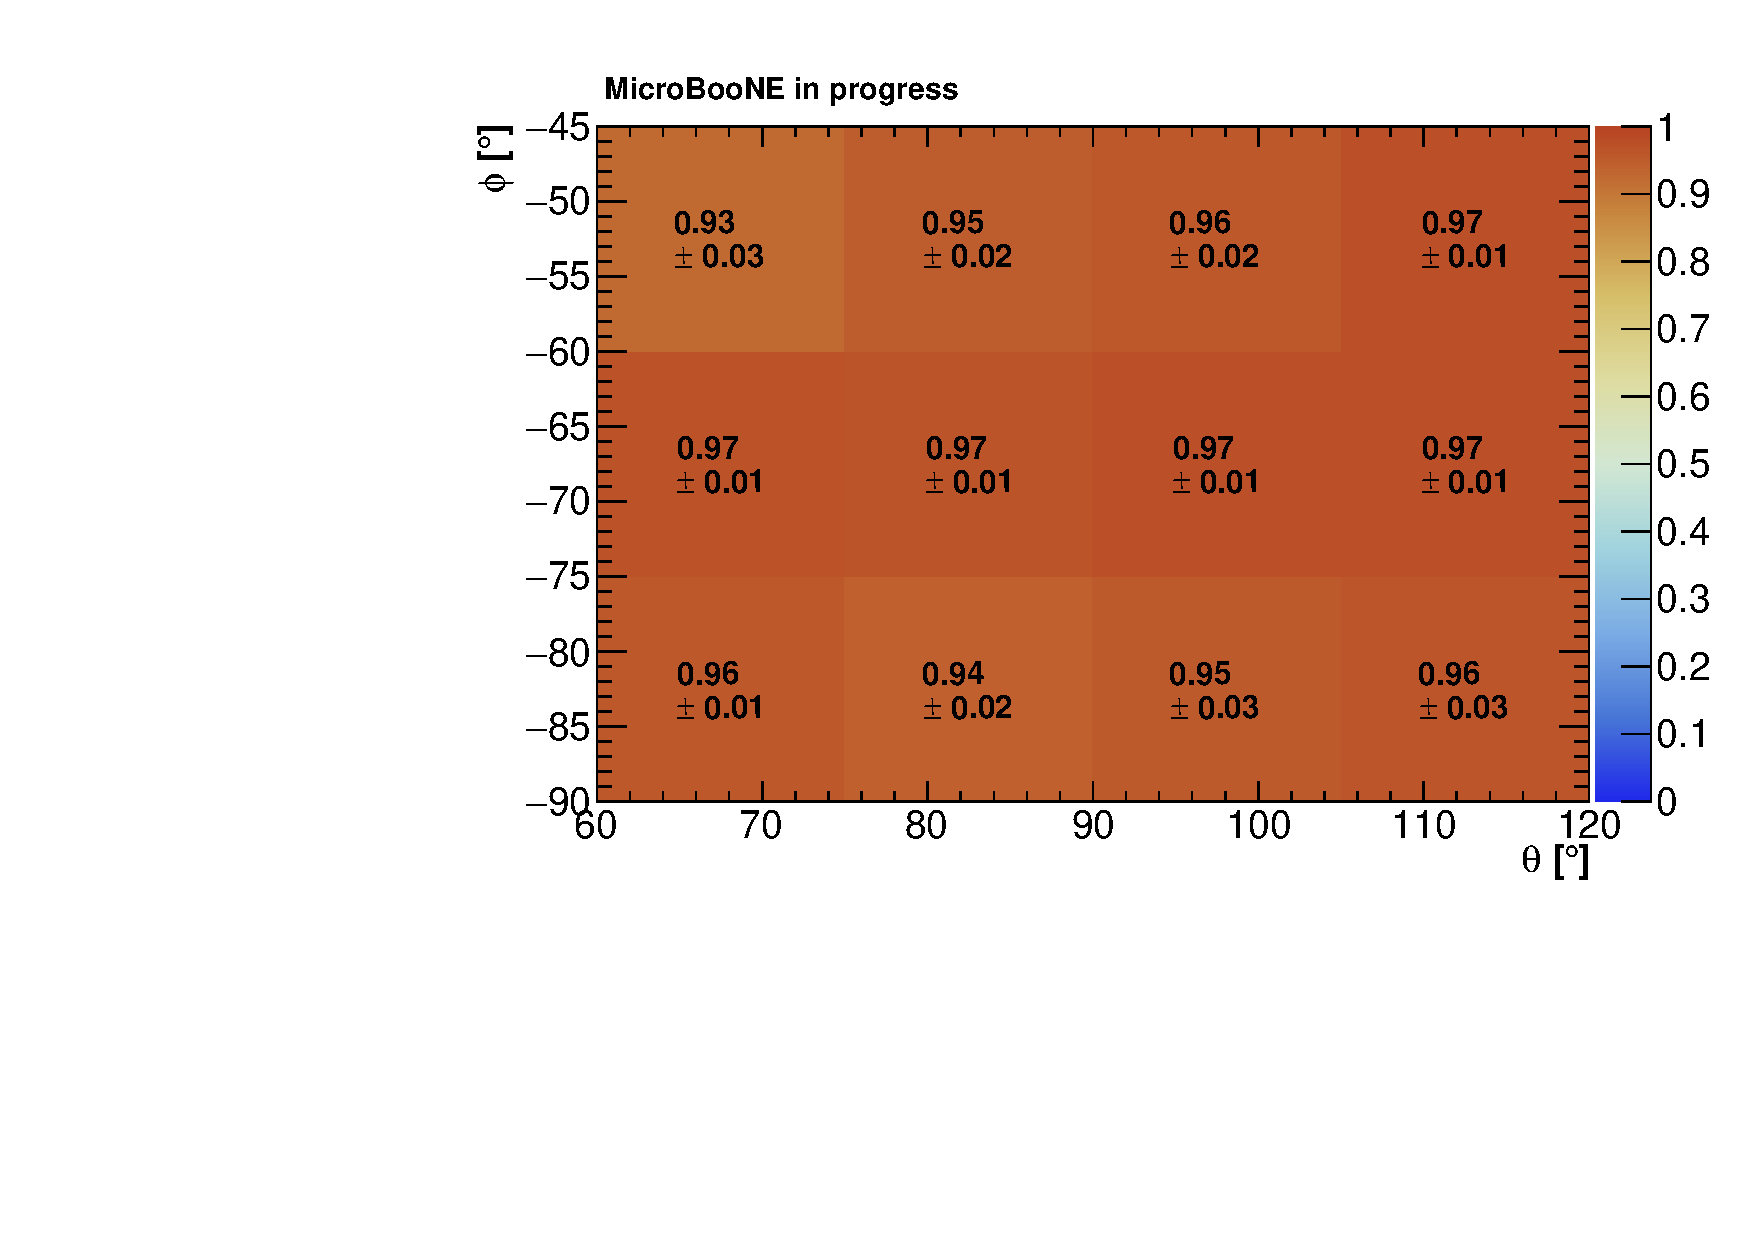
\includegraphics[width=\linewidth]{figures/e_theta_phi.pdf}
    \caption{$(\theta,\phi)$ - Data}
  \end{subfigure}\begin{subfigure}{0.33\textwidth}
  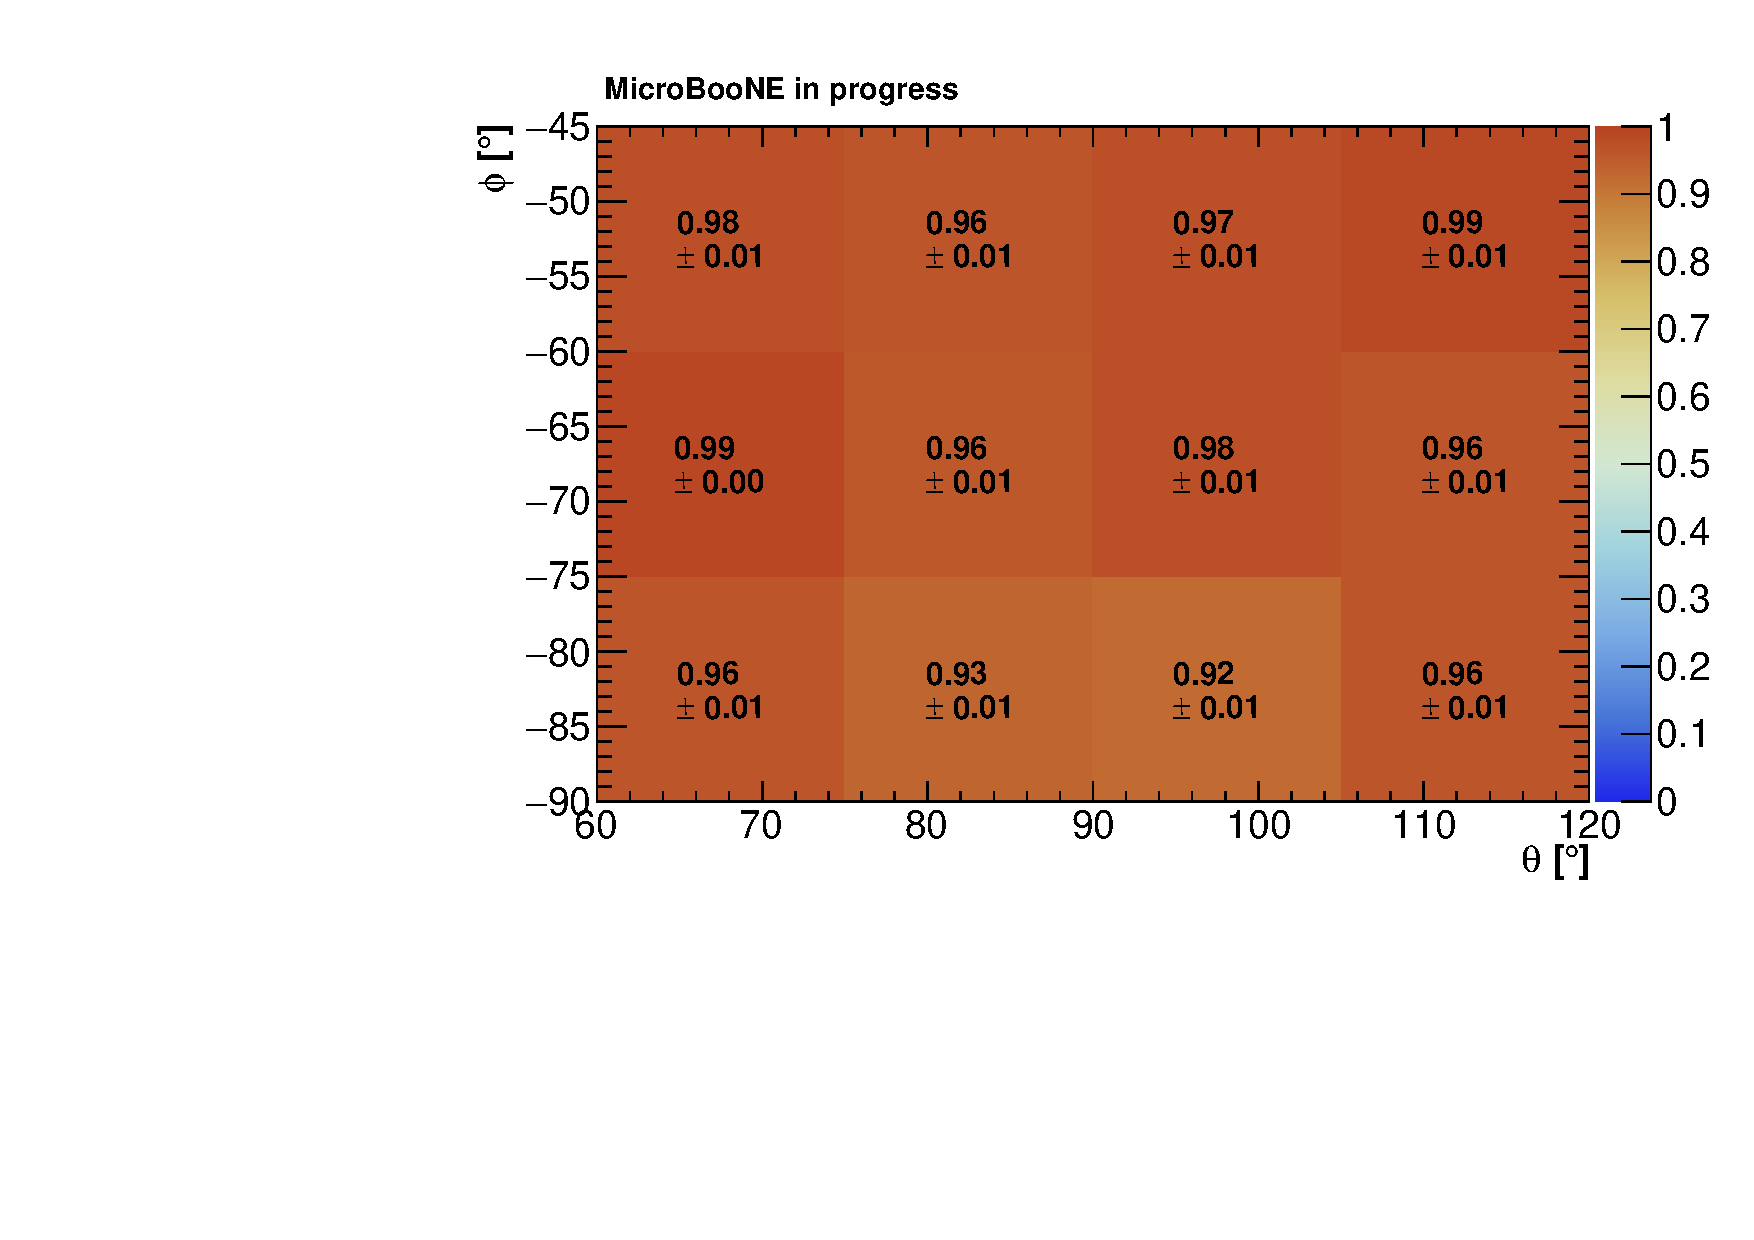
\includegraphics[width=\linewidth]{figures/theta_phi_mc.pdf}
  \caption{$(\theta,\phi)$ - Monte Carlo}
  \end{subfigure}\begin{subfigure}{0.33\textwidth}
  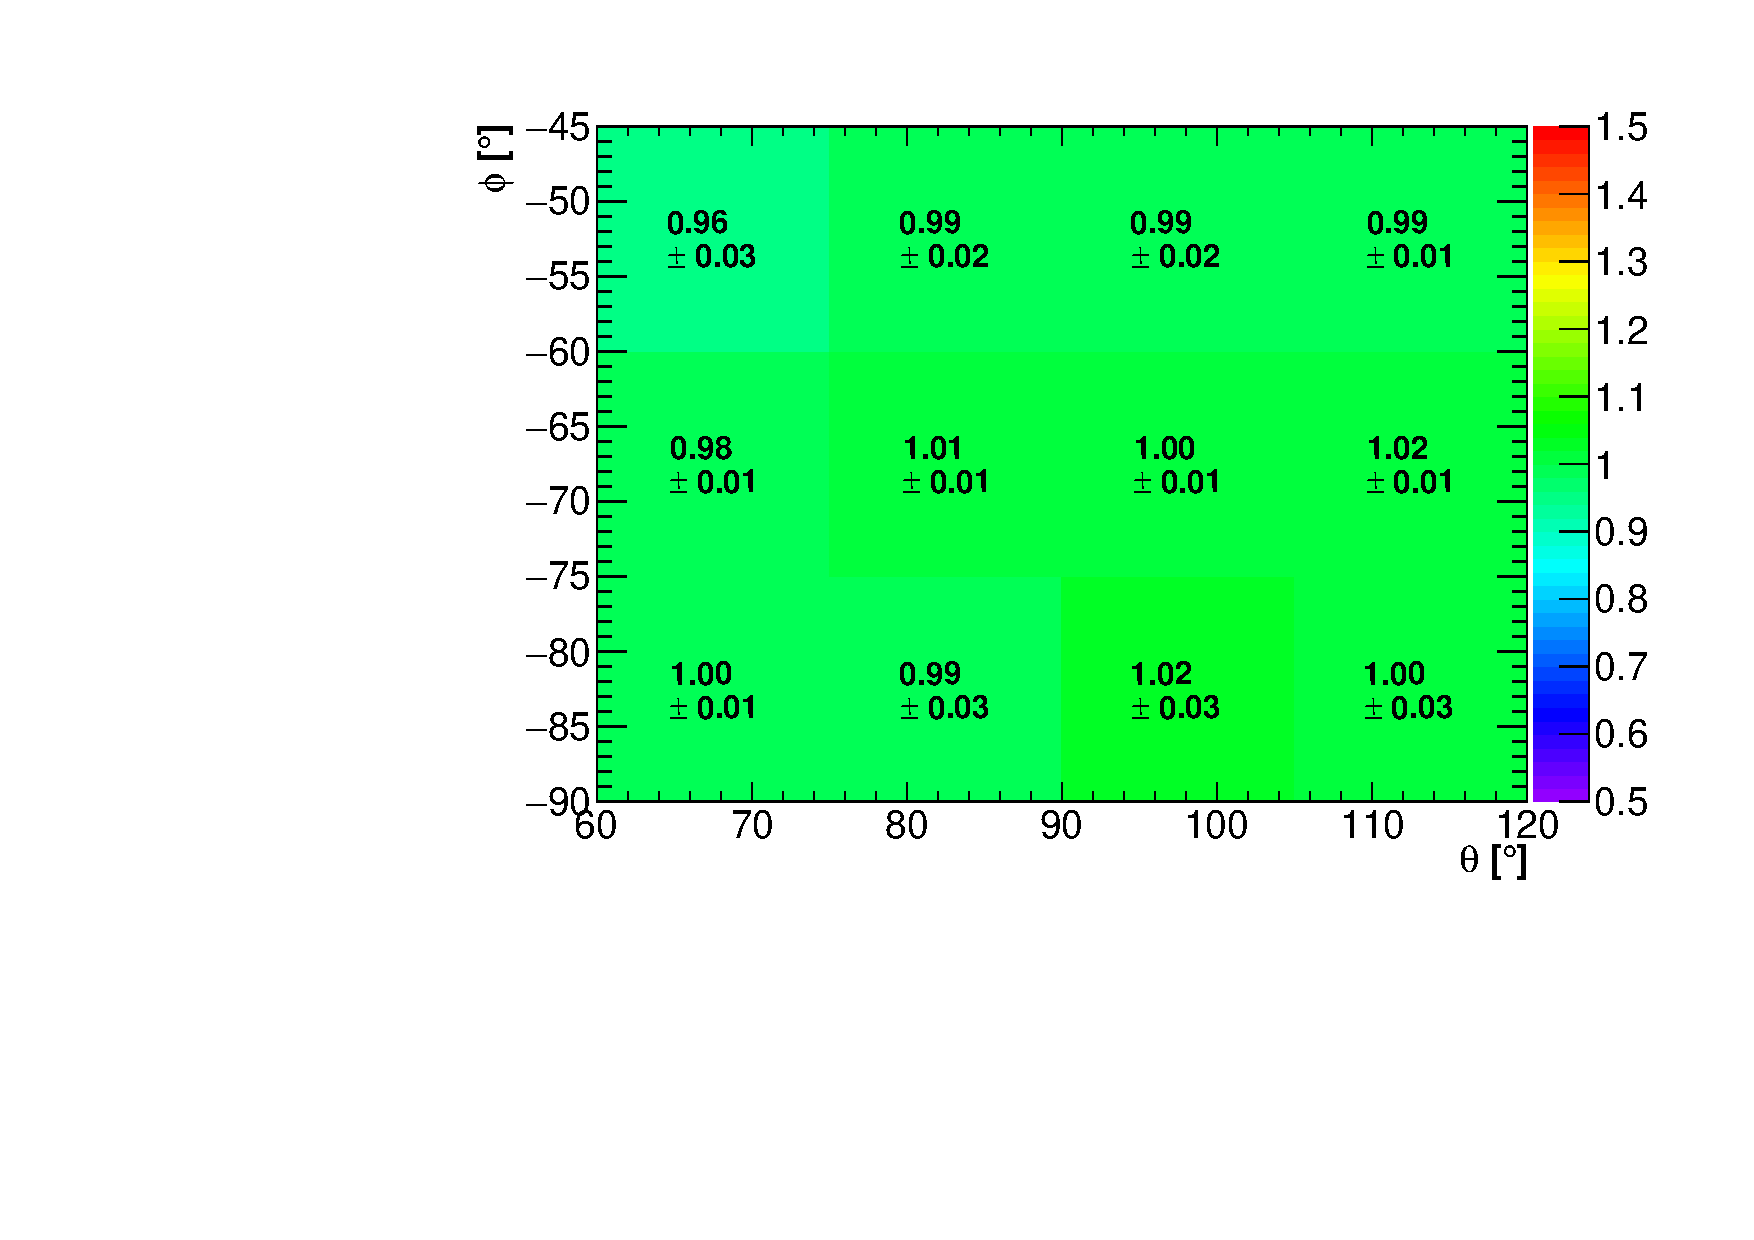
\includegraphics[width=\linewidth]{figures/theta_phi.pdf}
  \caption{$(\theta,\phi)$ - Data/Monte Carlo}
\end{subfigure}
\begin{subfigure}{0.33\textwidth}
  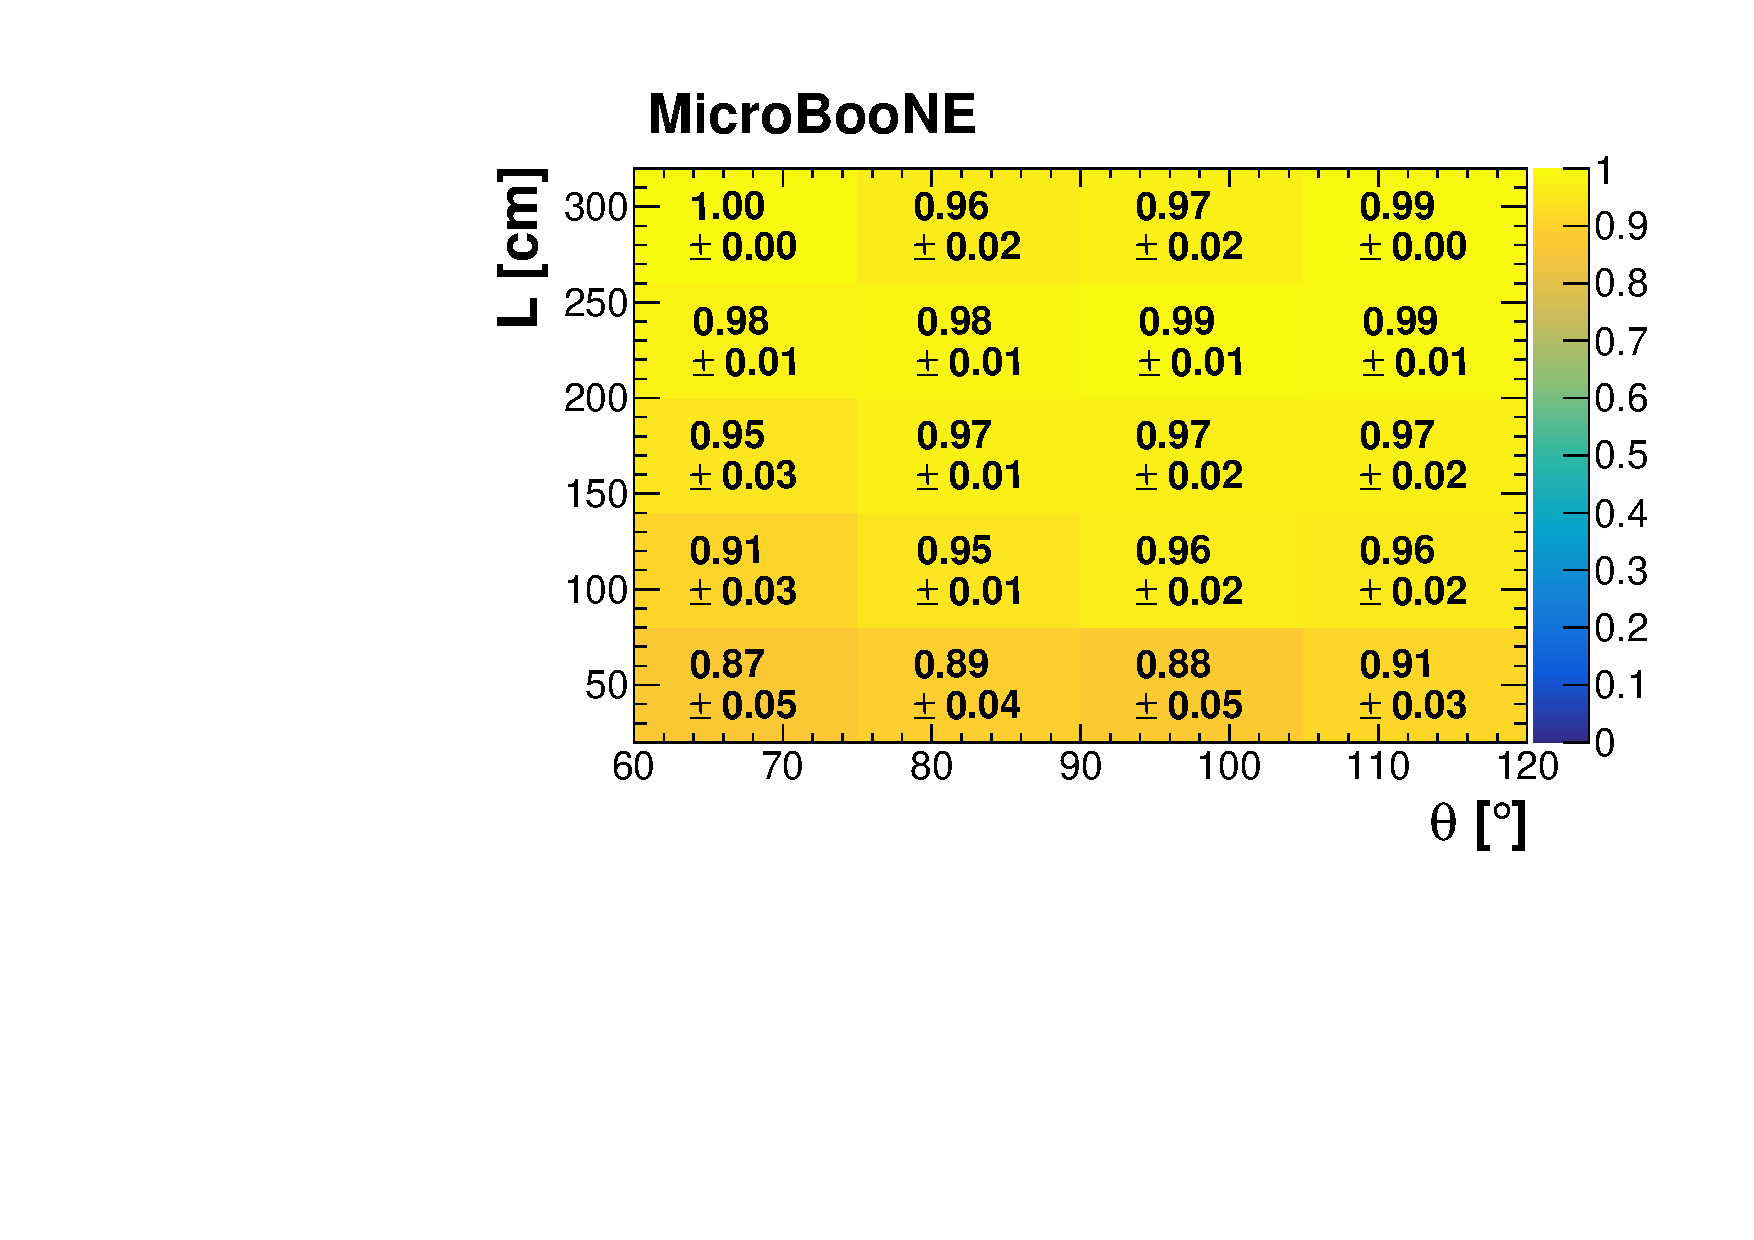
\includegraphics[width=\linewidth]{figures/e_theta_l.pdf}
  \caption{$(\theta,L)$ - Data}
\end{subfigure}\begin{subfigure}{0.33\textwidth}
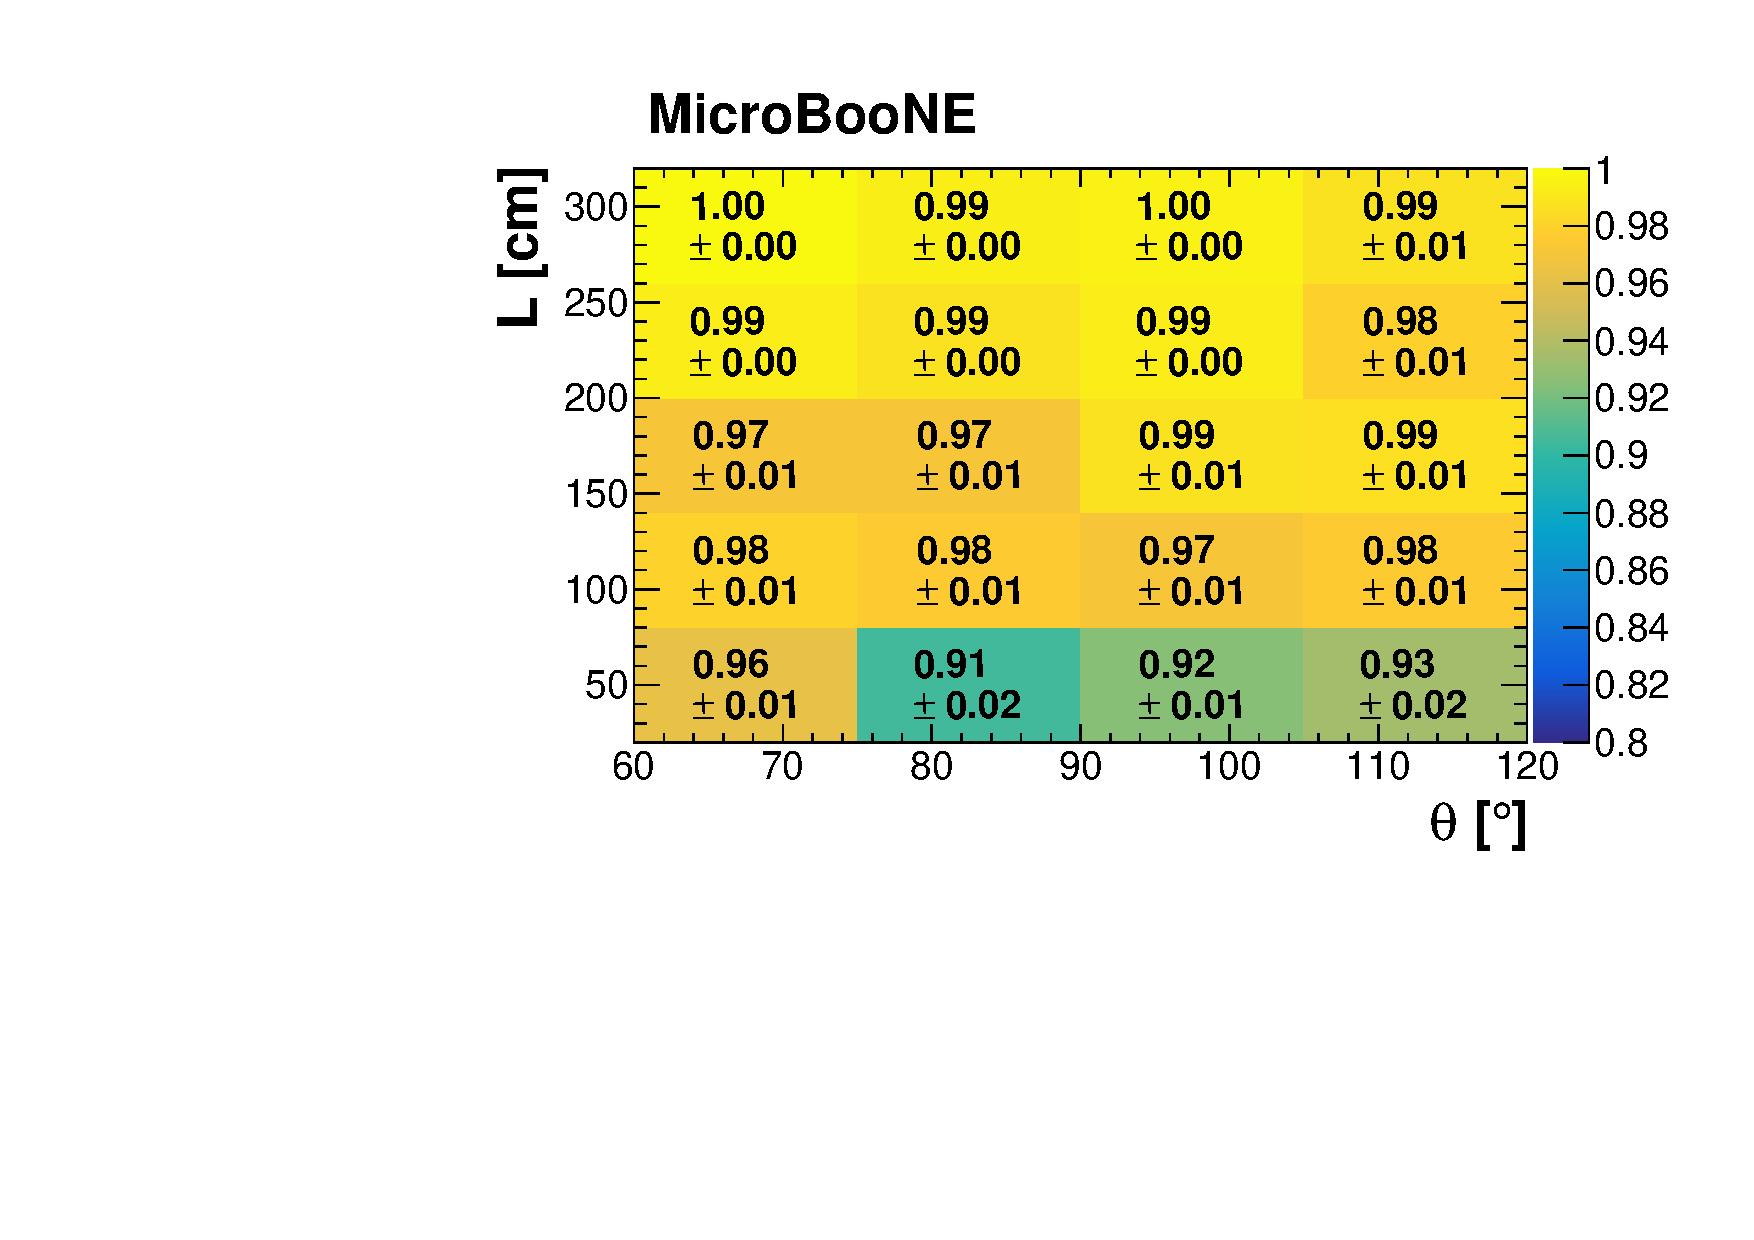
\includegraphics[width=\linewidth]{figures/theta_l_mc.pdf}
\caption{$(\theta,L)$ - Monte Carlo}
\end{subfigure}\begin{subfigure}{0.33\textwidth}
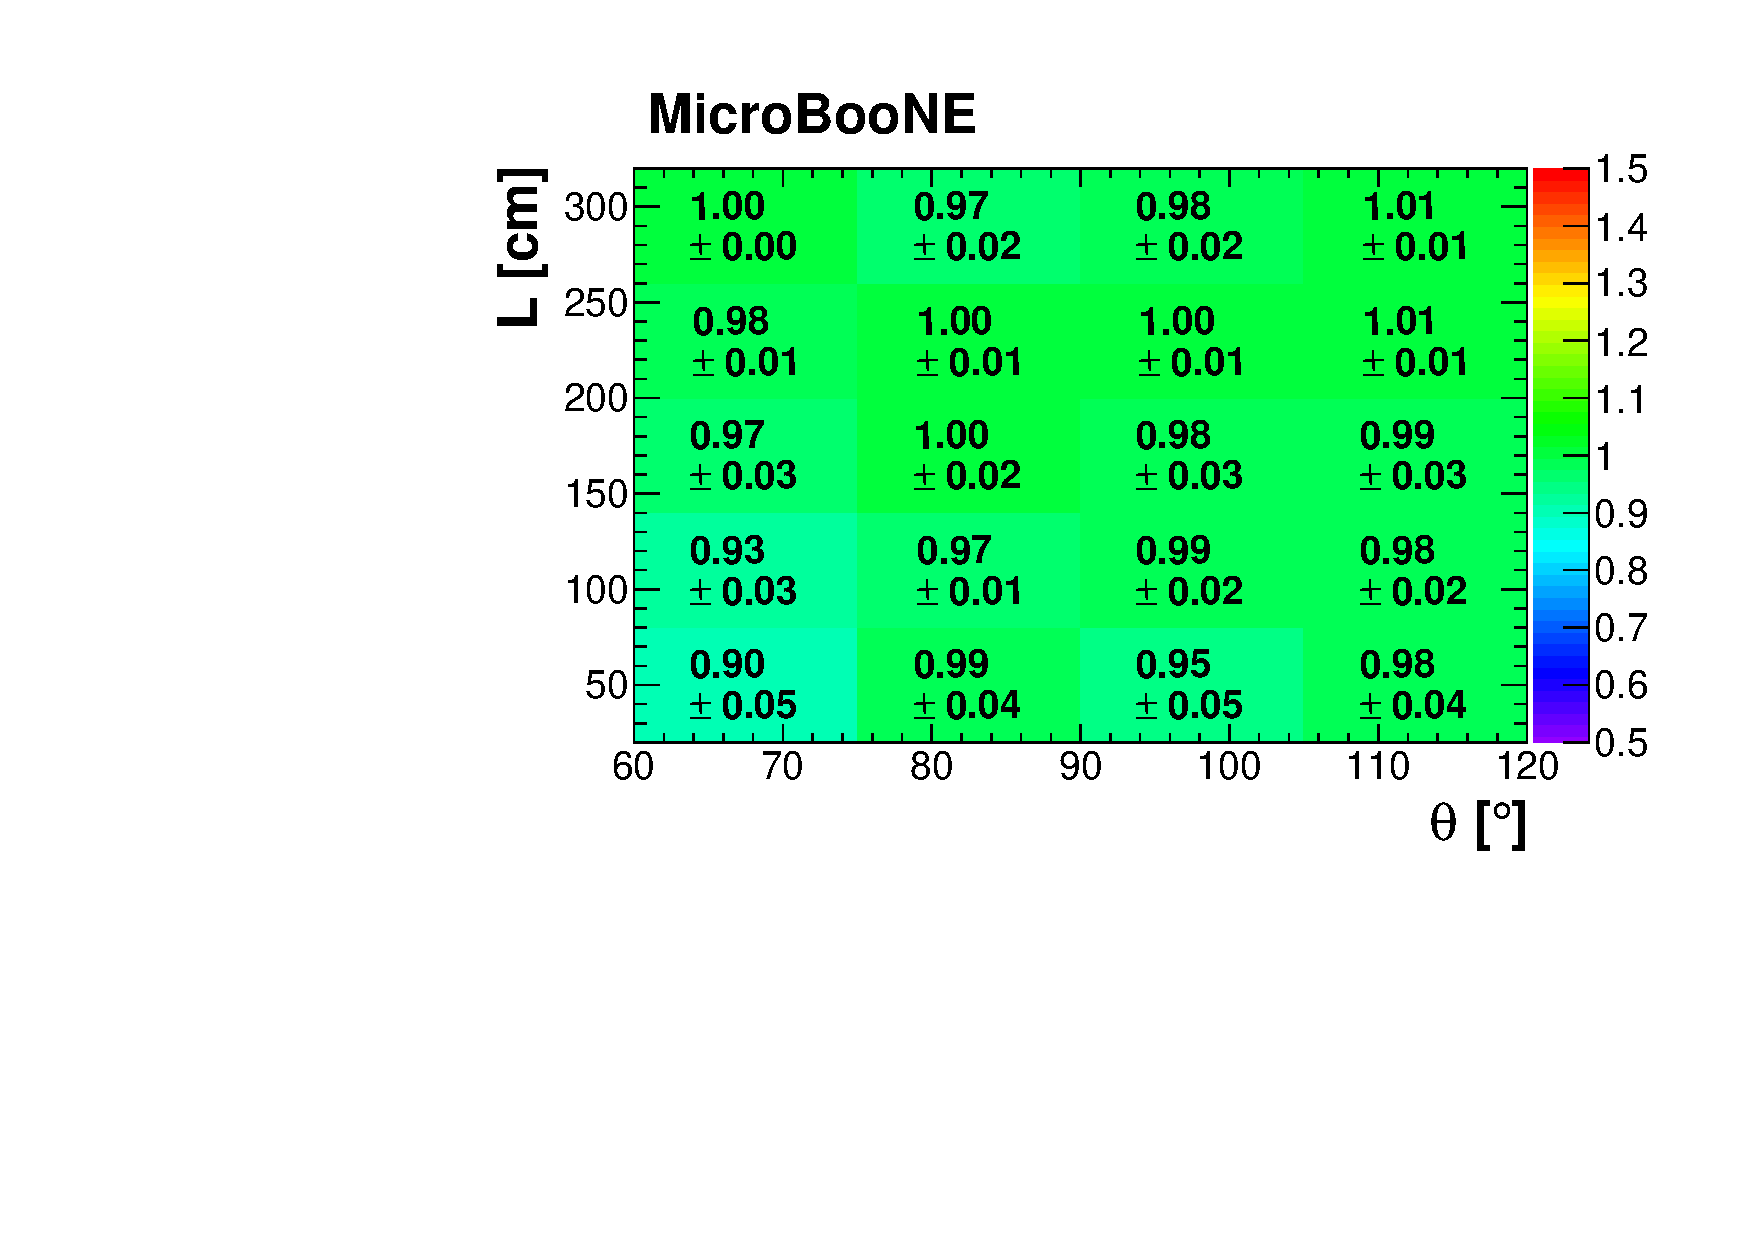
\includegraphics[width=\linewidth]{figures/theta_l.pdf}
\caption{$(\theta,L)$ - Data/Monte Carlo}
\end{subfigure}
\begin{subfigure}{0.33\textwidth}
  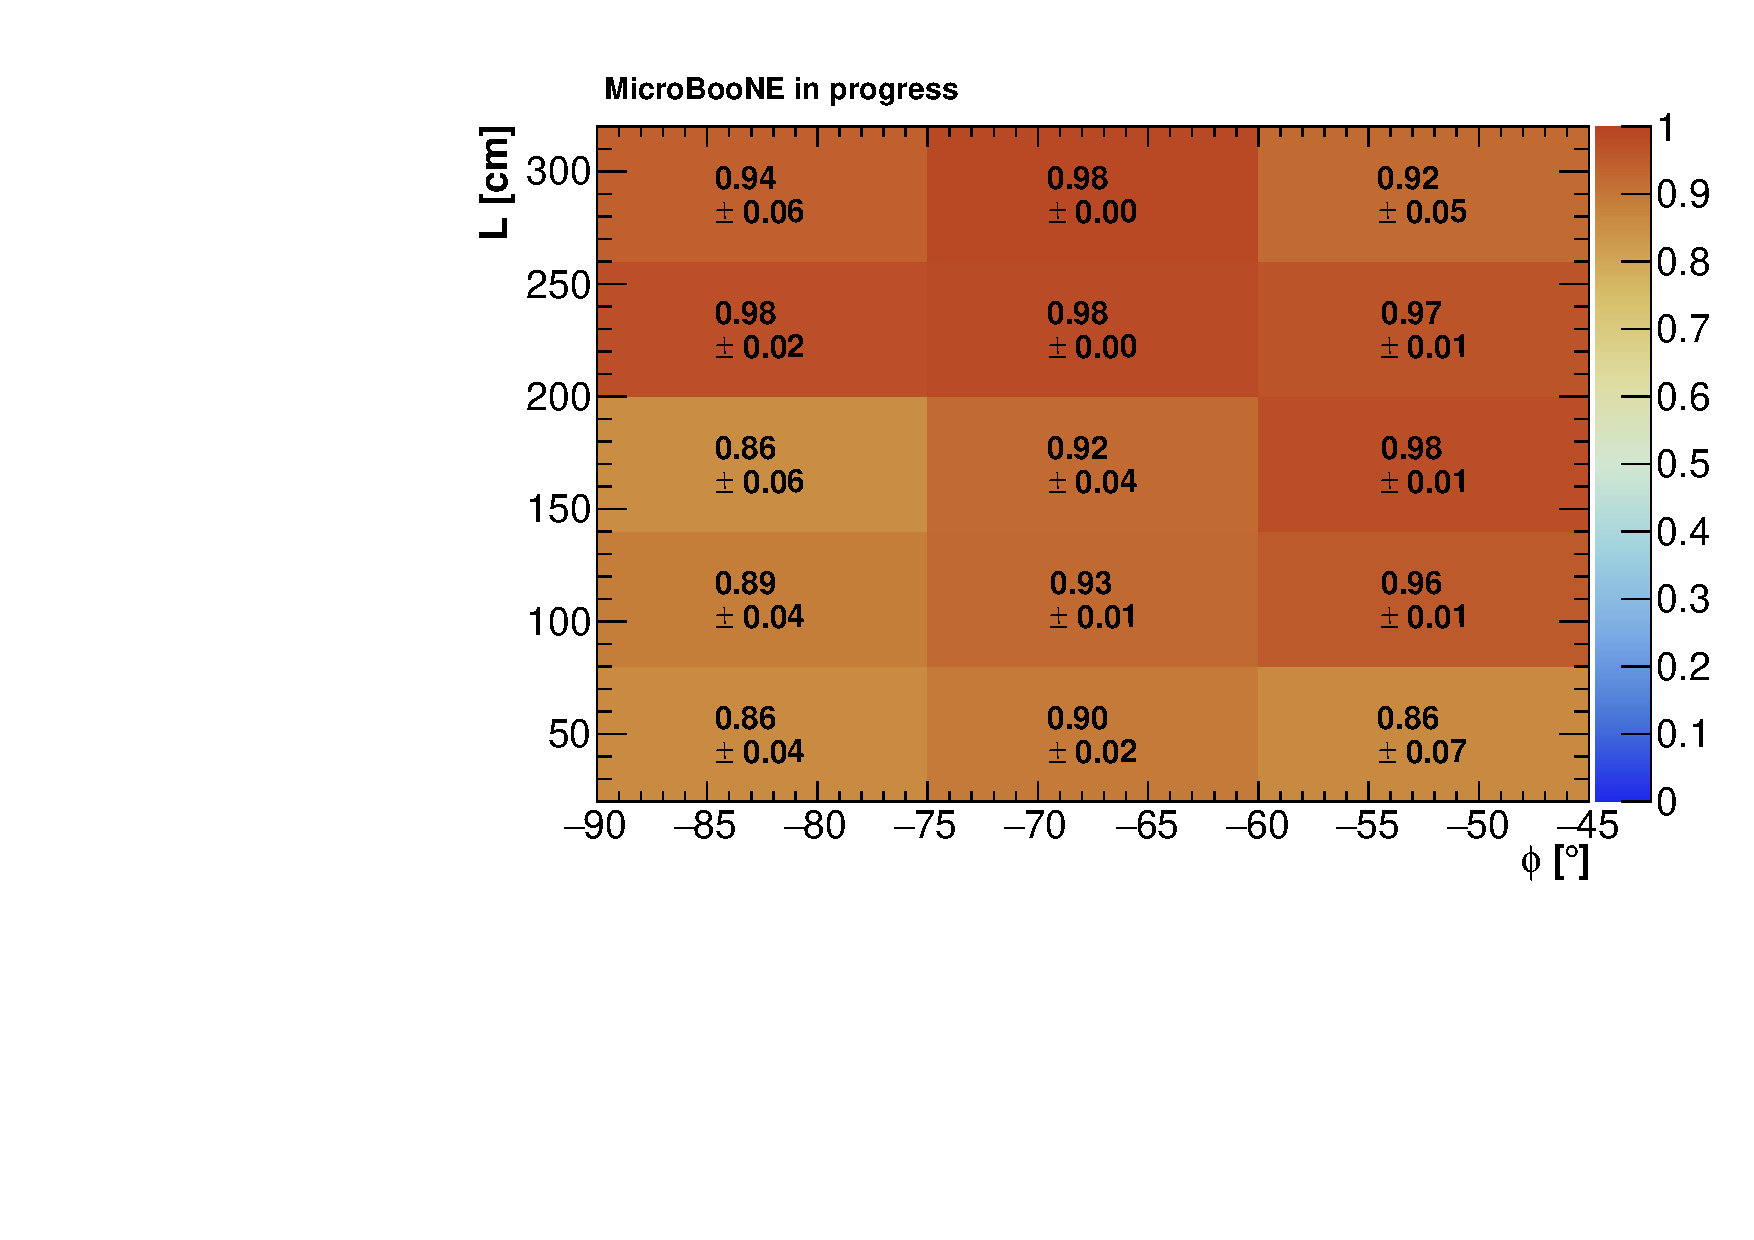
\includegraphics[width=\linewidth]{figures/e_phi_l.pdf}
  \caption{$(\phi,L)$ - Data}
\end{subfigure}\begin{subfigure}{0.33\textwidth}
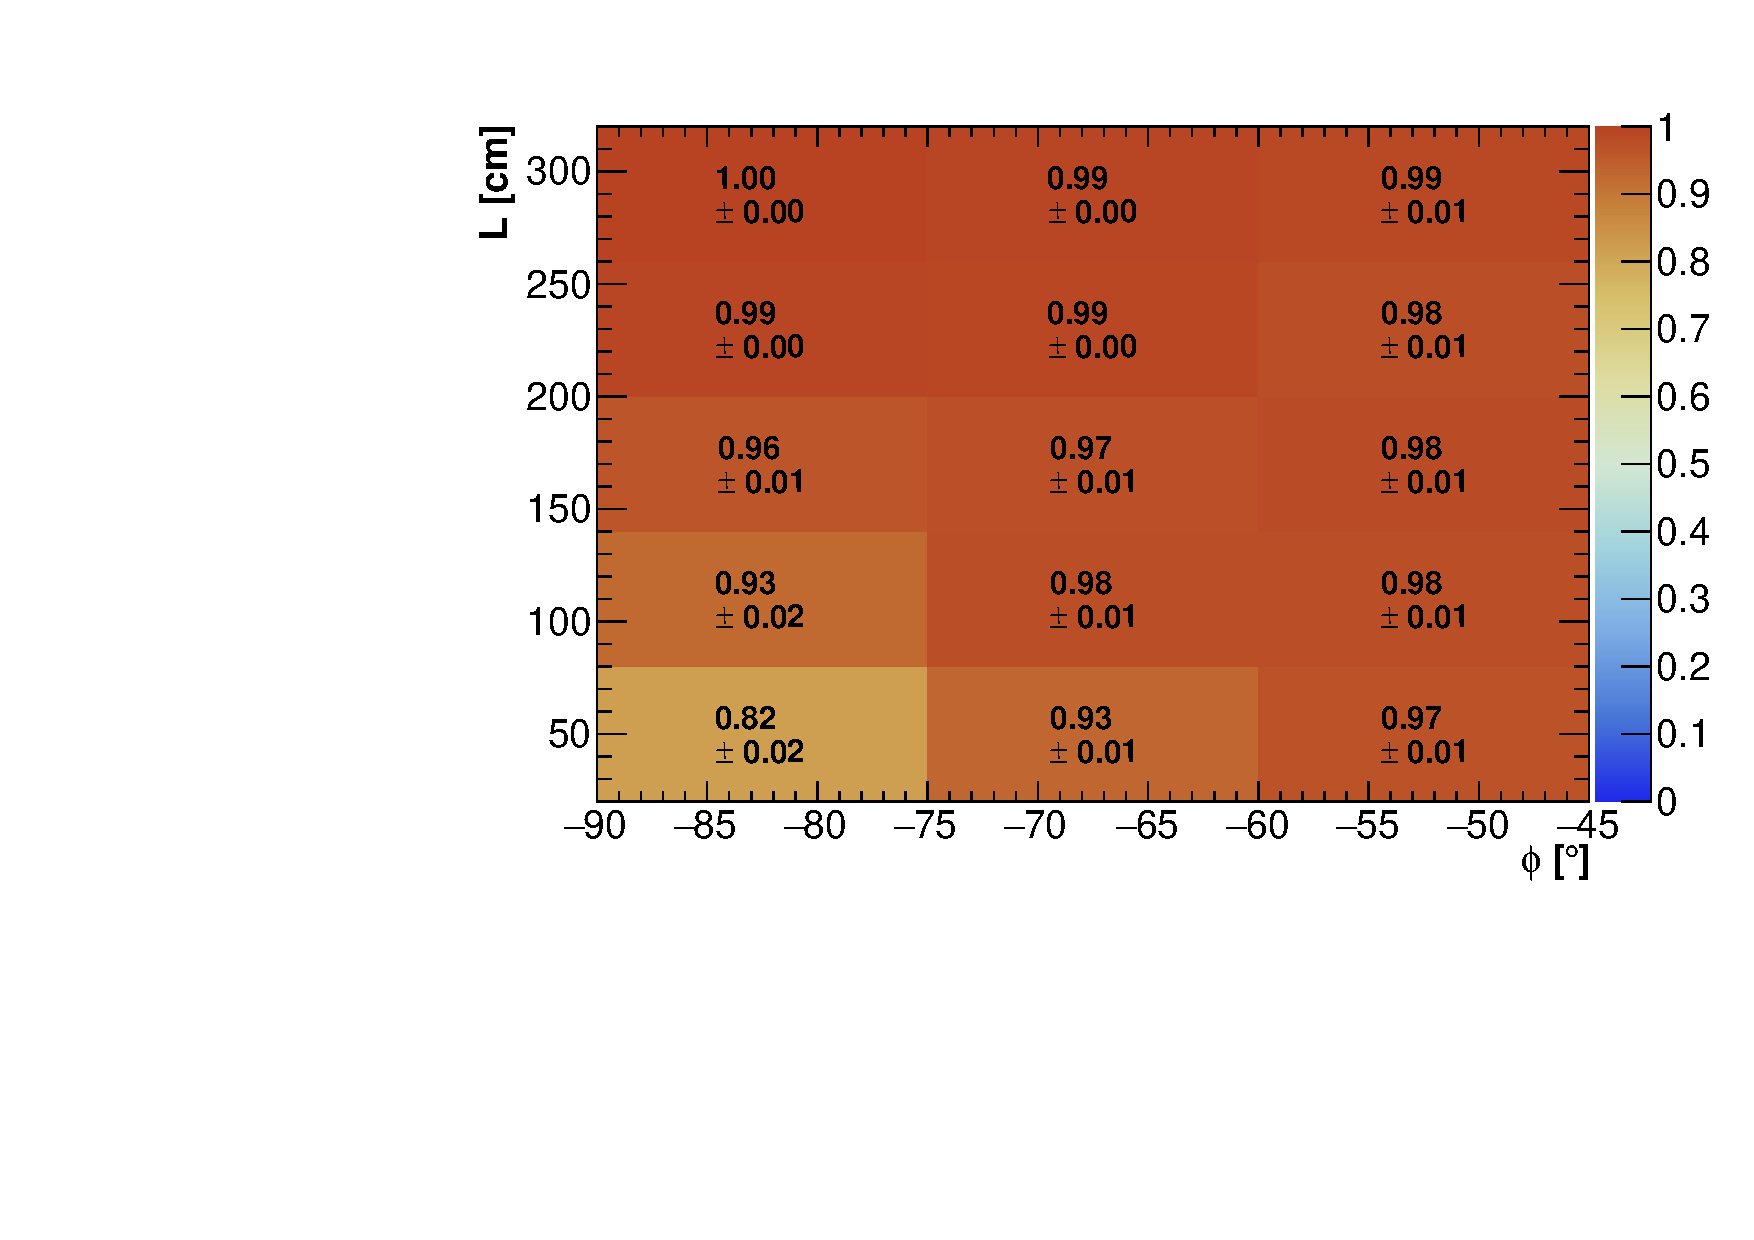
\includegraphics[width=\linewidth]{figures/phi_l_mc.pdf}
\caption{$(\phi,L)$ - Monte Carlo}
\end{subfigure}\begin{subfigure}{0.33\textwidth}
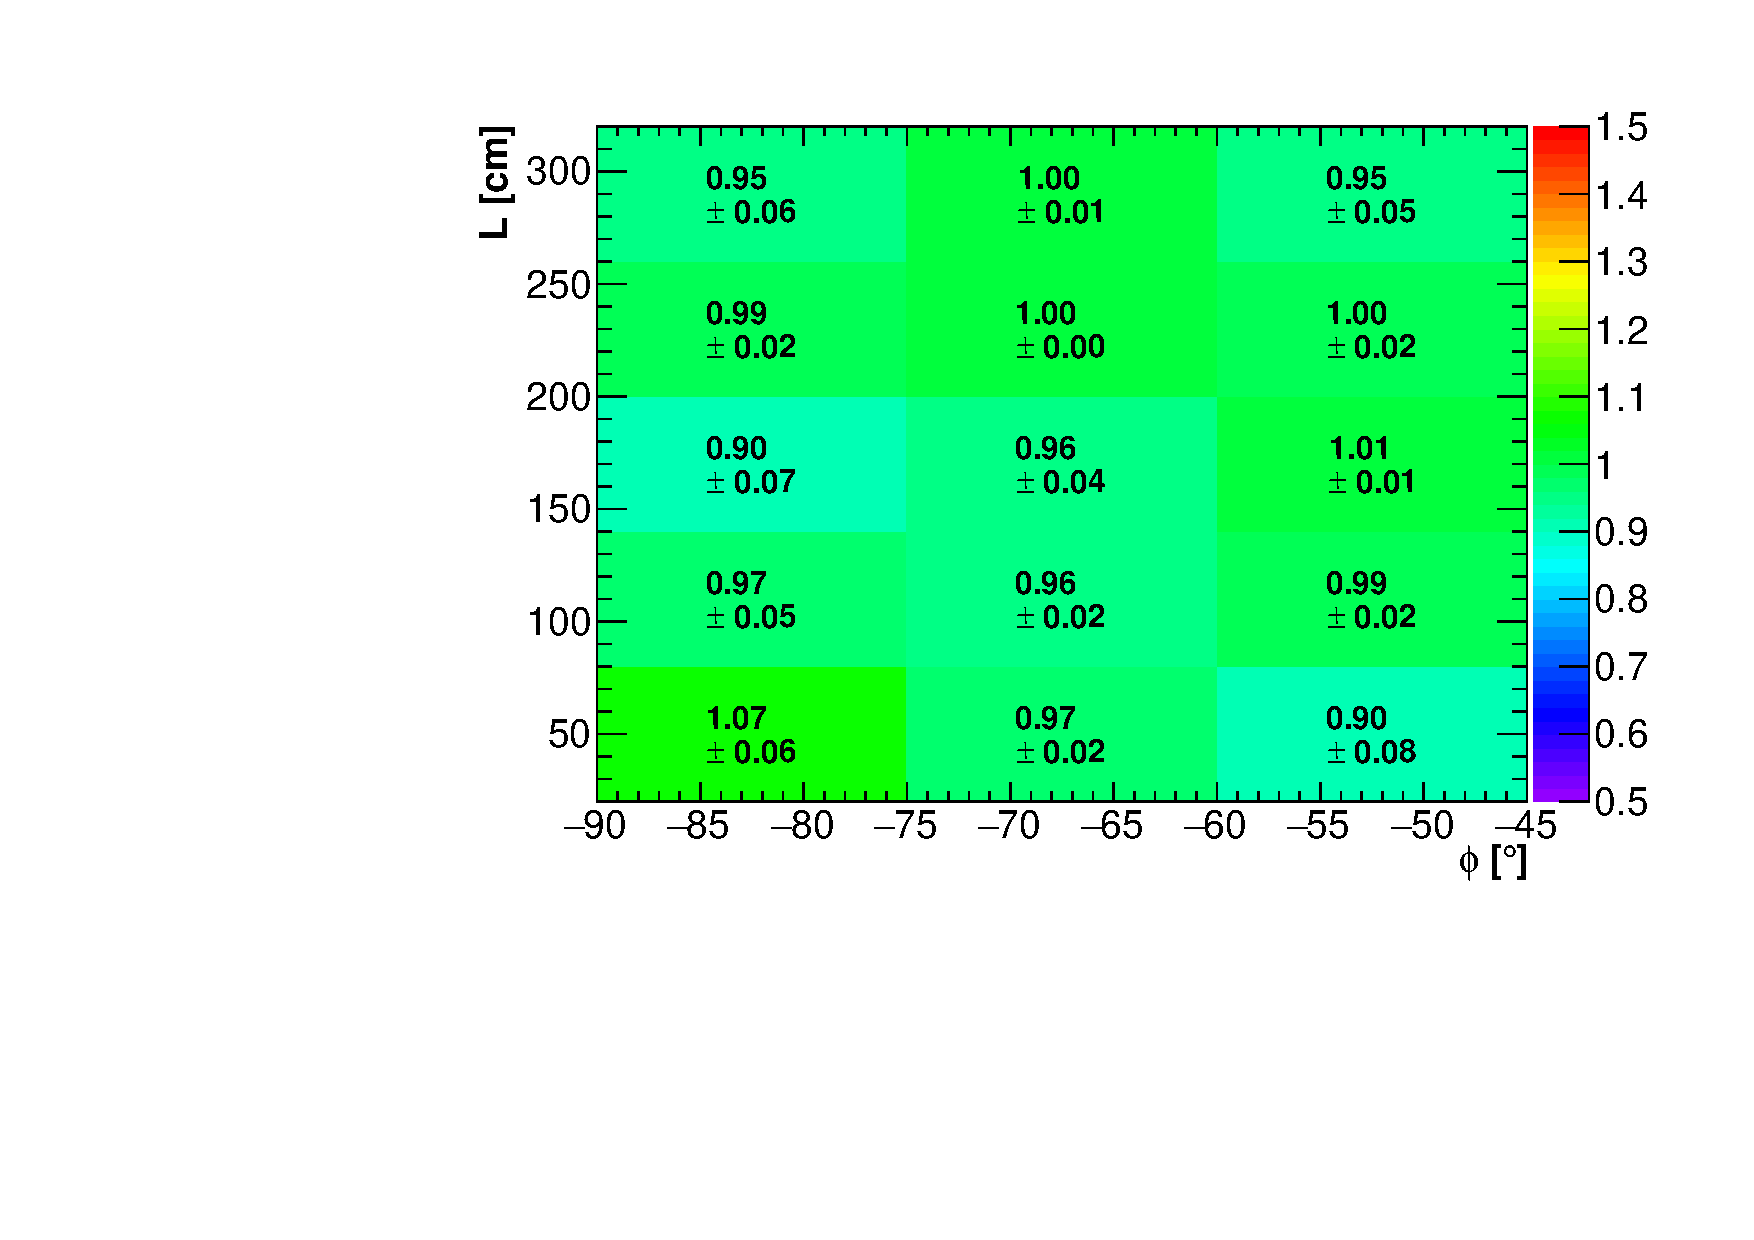
\includegraphics[width=\linewidth]{figures/phi_l.pdf}
\caption{$(\phi,L)$ - Data/Monte Carlo}
\end{subfigure}
\caption{Two-dimensional reconstruction efficiencies for data (left), Monte Carlo (center) and their ratio (right). Data errors include systematic effects.}\label{fig:2d}
\end{figure}

\section{Conclusions}
This analysis showed that it is possible to match hits in a muon counter system to a track in the LArTPC and that comparing the number of events triggered by the MuCS with the number of events with MuCS-tagged tracks we can measure the data reconstruction efficiency.

This efficiency, obtained with the procedure described in section \ref{sec:reco}, has been measured as a function of the starting angles $\theta$, $\phi$ and the expected length in the TPC, $L$. These coordinates have been measured using the spatial information provided by the hits in the MuCS.

The data reconstruction efficiency is in agreement, within the errors, with the Monte Carlo reconstruction efficiency, measured using a simulation of cosmic rays all over the LArTPC.

We have also shown that the detector non-uniformities must be taken into account in the measurement of the reconstruction efficiency and the related systematic error is 1.1\%.

However, the coverage of the ($\theta, \phi, L$) parameter space provided by the MuCS is limited and it is not possible to measure efficiency-corrected quantities, such as the cosmic-ray flux. The Cosmic Ray Tagger (CRT), assembled last summer, will be able to tag $\sim$80\% of the cosmic rays hitting the TPC and check the presence of non-uniformities in every part of the detector. Figure \ref{fig:crt} shows the coverage on the ($\theta,\phi$) plane of both the MuCS and the CRT, obtained with a Monte Carlo simulation.

\begin{figure}[htbp]
  \begin{center}
    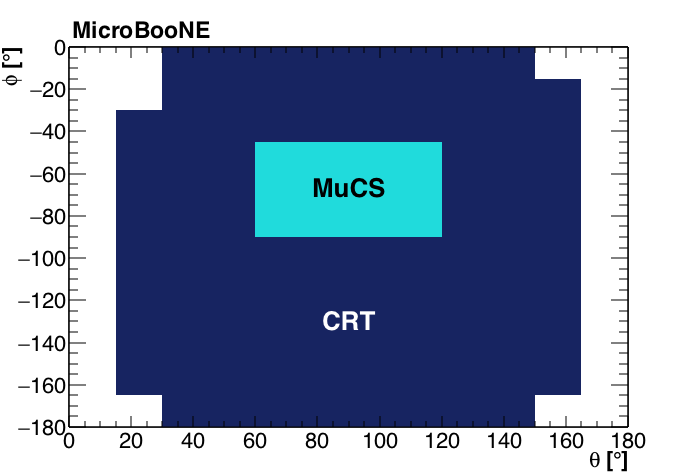
\includegraphics[width=0.7\linewidth]{figures/crt.png}
    \caption{Monte Carlo simulation of the coverage on the ($\theta,\phi$) plane of both the MuCS (light blue) and the CRT (dark blue).} \label{fig:crt}
  \end{center}
\end{figure}


\acknowledgments

This is the most common positions for acknowledgments. A macro is
available to maintain the same layout and spelling of the heading.



% We suggest to always provide author, title and journal data:
% in short all the informations that clearly identify a document.

\begin{thebibliography}{99}
  \bibitem{miniboone} A.~A.~Aguilar-Arevalo et al. [MiniBooNE Collaboration], \textit{Improved Search for $\bar \nu_\mu \rightarrow \bar \nu_e$ Oscillations in the MiniBooNE Experiment}, Phys.\ Rev.\ Lett.\  {\bf 110} (2013) 161801 \texttt{doi:10.1103/PhysRevLett.110.161801 [hep-ex/1303.2588]}.

  \bibitem{detector} R. Acciarri, et al. [MicroBooNE Collaboration], \textit{Design and Construction of the MicroBooNE Detector}, 2016  [\href{https://arxiv.org/abs/1612.05824}{\texttt{hep-ex/1612.05824}}].

  \bibitem{pandoracosmic} R. Acciarri, et al. [MicroBooNE Collaboration], \textit{The Pandora multi-algorithm approach to automated pattern recognition in LAr TPC detectors}, 2016  [\href{http://www-microboone.fnal.gov/publications/publicnotes/index.html}{MICROBOONE-NOTE-1015-PUB}].

  \bibitem{pandora} J.~S.~Marshall and M.~A.~Thomson, \textit{The Pandora Software Development Kit for Pattern Recognition}, Eur.\ Phys.\ J.\ C 75, no. 9, 439 (2015) \texttt{doi:10.1140/epjc/s10052\-015-3659-3} \texttt{[\href{https://arxiv.org/abs/1506.05348}{data-an/1506.05348}]}.

  \bibitem{crt} M. Auger, et al., \textit{A Novel Cosmic Ray Tagger System for Liquid Argon TPC Neutrino Detectors}, submitted to Instruments, \texttt{[\href{https://arxiv.org/abs/1612.04614}{ins-det/1612.04614}]}.

  \bibitem{mucs} S.R. Soleti, \textit{The Muon Counter System for the MicroBooNE experiment}, eConf C151216, \texttt{[\href{https://arxiv.org/abs/1604.07858}{ins-det/1604.07858}]}.

  \bibitem{mcdata} R. Acciarri, et al. [MicroBooNE Collaboration], \textit{A Comparison of Monte-Carlo Simulations and Data from MicroBooNE}, 2016 [\href{http://www-microboone.fnal.gov/publications/publicnotes/index.html}{MICROBOONE-NOTE-1014-PUB}].

  \bibitem{cosmic} R. Acciarri, et al. [MicroBooNE Collaboration], \textit{Cosmic Shielding Studies at MicroBooNE}, 2016 [\href{http://www-microboone.fnal.gov/publications/publicnotes/index.html}{MICROBOONE-NOTE-1005-PUB}].

  \bibitem{corsika} D.~Heck, et al.,
  \textit{CORSIKA: A Monte Carlo code to simulate extensive air showers}, 1998,
  \texttt{FZKA-6019}.

  \bibitem{geant} S.~Agostinelli, et al. [GEANT4 Collaboration], \textit{GEANT4: A Simulation toolkit}, Nucl.\ Instrum.\ Meth.\ A {506}, 250 (2003).

  \bibitem{sce} R. Acciarri, et al. [MicroBooNE Collaboration], \textit{Space Charge Effect Measurements and Corrections}, 2016 [\href{http://www-microboone.fnal.gov/publications/publicnotes/index.html}{MICROBOONE-NOTE-1018-PUB}].

  \bibitem{besiii} W.~L.~Yuan, et al., \textit{Study of tracking efficiency and its systematic uncertainty from $J/\psi \to p \overline{p} \pi^+ \pi^-$ at BESIII}, Chin.\ Phys.\ C 40 (2016) no.2,  026201 \texttt{doi:10.1088/1674-1137/40/2/026201}  \texttt{[\href{https://arxiv.org/abs/1506.05348}{hep-ex/1507.03453}]}.

  \bibitem{pdg} C.~Patrignani, et al. [Particle Data Group Collaboration], \textit{Review of Particle Physics}, Chin.\ Phys.\ C 40 (2016) no.10,  100001 \texttt{doi:10.1088/1674-1137/40/10/100001}.


% Please avoid comments such as "For a review'', "For some examples",
% "and references therein" or move them in the text. In general,
% please leave only references in the bibliography and move all
% accessory text in footnotes.

% Also, please have only one work for each \bibitem.


\end{thebibliography}
\end{document}
